\documentclass[preprint,review,12pt]{elsarticle}

\usepackage{amsmath}

\usepackage{amsfonts}
\usepackage{graphicx}
\newcommand{\Rho}{\mathrm{\textit{P}}}
\usepackage{subcaption}
\usepackage{csquotes}
\usepackage{algorithm} 
\usepackage{algpseudocode} 
\usepackage{longtable}
\usepackage[top=1.0in, bottom=1.0in, left=1.0in, right=1.0in]{geometry}
\usepackage{url}
\def\UrlBreaks{\do\/\do-}
\usepackage{breakurl}
\usepackage[breaklinks]{hyperref}
\begin{document}

\begin{frontmatter}


\title{Who You Gonna Believe, Me or Your Lying Eyes?\\
An Epidemiological Examination of Fake News and a Ranked Solution}

\author{By \\\textbf{John Hawthorne Smith} \\Thesis Project \\Submitted in partial fulfillment of the \\requirements for the degree of \\ \\MASTER OF SCIENCE IN DATA SCIENCE \\ \\Northwestern University \\April, 2021 \\ \\Nathaniel D. Bastian, PhD, First Reader \\Syamala Srinivasan, PhD, Second Reader}




\begin{abstract}
%% Text of abstract
Within the past decade, social media has become a primary platform for consumption of information and current events. Unlike with traditional news sources, however, social media posts do not have to go through a rigorous validation process prior to publication. The 2019 Mueller Report illustrates how malicious actors have taken advantage of these lax requirements to sway public opinion on topics from the \#blacklivesmatter movement to the 2016 U.S. Presidential election. 

Currently, social media companies rely primarily on communal-policing of misinformation: this is unlikely that this will happen with regularity. To counteract this, other literature on the topic is focused on building neural networks that will be able to detect accurate from misleading content; however, the rapidly evolving nature of misinformation means that they will have to be retrained and redeployed on an iterative and time-consuming basis.

This thesis, therefore, proposes a novel approach to the problem: treating misinformation as a virus. This thesis proposes a ranking system that third-party fact checkers can utilize to prioritize posts for checking. This algorithm is then tested against multiple data sets with strong positive results, decreasing viral spread in a matter of minutes.

\end{abstract}

\begin{keyword}
%% keywords here, in the form: keyword \sep keyword
Social media \sep Fake news \sep Misinformation \sep Partisanship \sep Networks
\end{keyword}

\end{frontmatter}

\section{Introduction}
\label{introduction}
 In 2018, social media overtook print media as the fourth most popular source of news for Americans. As of 2019, 20\% ``often" got their news from social media \cite{shearer2018social}, while 68\% of all American got their news from social media at least occasionally \cite{matsa2018news}. This is not inherently a bad thing - in countries with authoritarian leaders and state-run media, social media may be the only outlet for opposition spokespeople to share their messages \cite{walker2014breaking}; ordinary citizens can now contribute their stories and experiences without the high financial barrier to entry that traditional journalism requires \cite{qualman2012socialnomics, tapscott2008wikinomics}; in unmanageable situations and crises, such as the 2017 Manchester bombing, social media allows for the instantaneous exchange of information between individuals and emergency management agencies \cite{mirbabaie2020breaking, eriksson2016facebook}; in situations like the COVID-19 pandemic, where information is rapidly evolving, social media allows for immediate knowledge dissemination by dramatically shortening the traditional time from publication to widespread translation to adoption \cite{chan2020social}. 
 
However, not all information shared on social media is true, and the subset of people who primarily get their news from social media tend to be less engaged, less knowledgeable of current events, more likely to hear unproven claims and conspiracy theories than those who get their news from more traditional sources, and are more likely to believe these conspiracies \cite{mitchell2020americans}. In just two examples of this, Edgar Maddison Welch drove from North Carolina to Washington D.C. with an AR-15 to investigate a fake pedophile conspiracy ring known as ``pizzagate" in December 2016, \cite{goldman2016comet}; in 2018, Burmese officials created over 1,000 Facebook posts filled with hate speech and detailing fake crimes committed by the Rohynga Muslim minority to justify one of the largest forced migrations in recent history \cite{subedar2018country}.

Exacerbating this problem, the spread of correct information is much slower than that of misinformation: while true rumors tend to be validated within 2 hours of the first tweet, false rumors take about 14 hours to be debunked \cite{zubiaga2016analysing,shao2016hoaxy}. This is a problem since, in a crisis event, 50\% of all retweets occur within the first hour after a tweet is shared and 75\% are within the first day \cite{kwak2010twitter}. Even if an untrue story is debunked, corrective information does not reach as broad of an audience as misinformation does \cite{maddock2015characterizing, vosoughi2018spread}, and, in some cases, rumors and other fake stories actually see an increase in spread \textbf{after} they have been debunked \cite{starbird2014rumors}. In fact, this fits a pattern where highly controversial and politicized topics spark backfire effects when passionately held misconceptions are challenged \cite{gollust2009polarizing,nyhan2010corrections,nyhan2013hazards,redlawsk2010affective,schaffner2016misinformation,hart2012boomerang}.

\subsection{Problem Statement}
\label{Problem Statement}
A reasonable person might still question at this point why this is a problem that needs solving. There is nothing fundamentally new and original about lying, especially on controversial or political topics. While this is true, it is imperative not to sink into an \textit{argument from inertia} fallacy and suggest that because history has survived this issue in the past, there is no reason to improve in the present \cite{bennett2012logically}. Arguably, there are three major reasons to try to prevent the spread of fake news: the legal, the ethical, and the humanitarian.

While it is true that the US Supreme Court has routinely ruled in favor of providing more freedom than less when it comes to speech, false statements with dire consequences do not fall under those rulings. 
In \textit{Garrison v. Louisiana}, the Court unequivocally stated ``[T]he knowingly false statement and the false statement made with reckless disregard of the truth, do not enjoy constitutional protection" \cite{scotus1964garrison} and in \textit{Hustler v. Falwell}: ``[f]alse statements of fact are particularly valueless [because] they interfere with the truth-seeking function of the marketplace of ideas" \cite{scotus1987hustler}. These quotes are the guiding principle of this article: it is not the intention of this algorithm to remove bad ideas from the marketplace, but to remove bad faith ideas.

In book one of \underline{Metaphysics of Morals}, Immanuel Kant argued that the great injustice of lying is that it robs the person being lied to of the freedom to make their own decisions \cite{kant1996metaphysics}. By operating with an incomplete or incorrect set of facts, a virtuous and rational person could make an unethical and misguided decision that they would not have made otherwise. This is not dissimilar from the arguments made in the Mueller report and in the indictment against the IRA: Count One was ``conspiracy to defraud the United States" in order to interfere in the 2016 election  \cite{mueller2019mueller,mueller2020internet}. The primary goal of the IRA, per Mueller, was to sow confusion -- getting individuals to accept the fraud was a bonus -- and make people unsure of which sources, if any, they could trust. That goal was successful, since 64\% of Americans believe that fake news causes a great deal of confusion and roughly 1 in 4 admit to having shared fake stories themselves \cite{barthel2016americans}. Those rates of confusion are relatively consistent across the political spectrum, gender, income levels, etc. 

One example of a Russian fraud account is @TEN\_GOP (fig. \ref{fig:Russian Troll Account @TEN_GOP}), \begin{figure}[h]
    \centering
    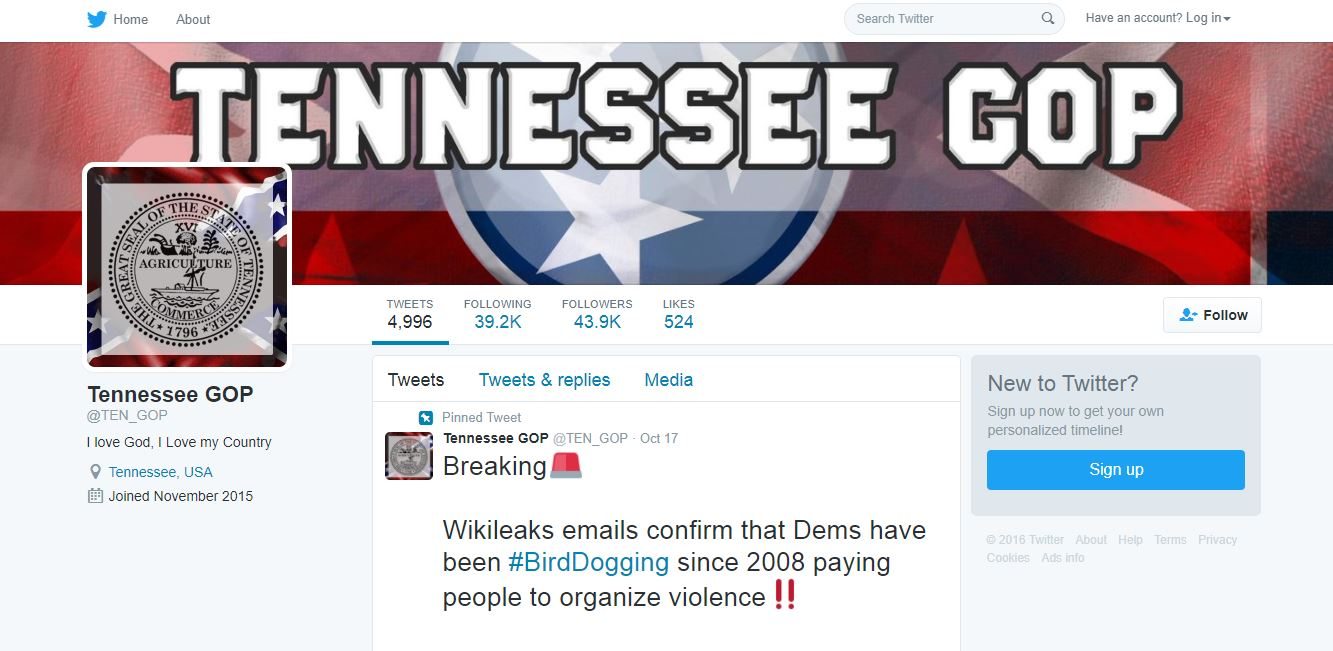
\includegraphics[width=11cm]{Ten_GOP.jpeg}
    \caption{@TEN\_GOP, Russian Troll Account}
    \label{fig:Russian Troll Account @TEN_GOP}
\end{figure} which is mentioned repeatedly in the Mueller report and claimed to be the official twitter of the Tennessee Republican Party. It racked up over 100,000 followers and frequently shared false information regarding voter fraud which was then retweeted by multiple individuals key to the Trump campaign \cite{mueller2019mueller}. As will be discussed later in \ref{Partisanship Section}, individuals will conform to the opinions of the rest of a group, even if it runs contrary to their personal convictions or facts they've personally observed \cite{asch1956studies}, especially in politically charged environments \cite{bullock2007experiments,housholder2014facebook}. This is the heart of the ethical objection: misinformation intends, at its core, to exploit human weakness and rob individuals of the freedom to make informed decisions.

The humanitarian arguments are the most important reasons for curbing the spread of disinformation. A prime example is the ``pizzagate" story where a person brought an AR-15 into a restaurant, but this is far from a unique example. Hours after the 2013 Boston Marathon Bombing, members of social media hypothesized that an innocent Brown University student was behind the attack \cite{starbird2014rumors}; he committed suicide shortly after. A father of a child who was killed during the 2012 Sandy Hook shooting was harassed by social media members convinced that the shooting was a hoax \cite{williamson2019alex}; he too committed suicide shortly after. On January 6, 2021, incited by the former President of the United States's debunked claims over election fraud, a mob broke into the U.S. Capitol and threatened to execute members of Congress and the Vice President \cite{fandos2021trump}; five people were killed directly from riot \cite{Levenson2021capitol}.

\subsection{Fake News Definition}
\label{Fake News Definition Section}
Before continuing, it's important to get a clear definition of what is meant by the term ``fake news". The primary and most frequently cited definition of fake news comes from Allcott \& Gentzkow: ``[they are] articles that are intentionally and verifiably false, and could mislead readers" \cite{allcott2017social}. Several existing studies adopt this definition \cite{conroy2015automatic,klein2017fake,rubin2015deception,rubin2017deception,mustafaraj2017fake,potthast2017stylometric}, and most attempt to parse out the further differences between \textit{misinformation}, \textit{disinformation}, \textit{rumor}, \textit{fake news}, etc. \cite{zimdars2020fake,  difonzo2007rumor,flynn2017nature,garrett2013undermining,wu2016mining}. Wu et al. provide the following diagram of their proposed parsing:
 \begin{figure}[htp]
    \centering
    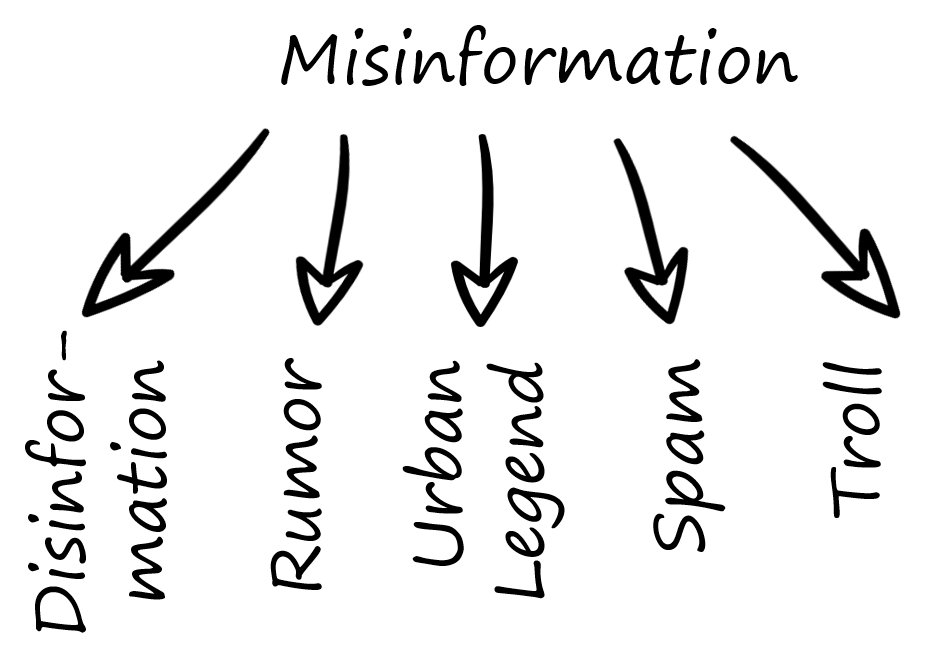
\includegraphics[width=4cm]{misinformation graphic.png}
    \caption{Misinformation Labels \cite{wu2016mining}}
    \label{fig:misinformation graphic.png}
\end{figure}


The dividing line between most of these categories is the level of intentionality, which has lead to an alternative definition from Klein \& Wueller: ``[misinformation is] a news article that is intentionally and verifiably false". \cite{klein2017fake}. This definition has seen growth and has also been accepted by current studies \cite{shu2017fake, liu2018early}.

Here, a more epistemological approach is proposed. For every tweet $t$ in the set of tweets $T$, there is a corresponding truth value $\tau$ between 0 and 1 (0 means something is completely false and 1 means something is completely true): $\forall \ t \in T \ \exists \ \tau, \tau \in \mathbb{R} \ | \ 0 \leq \tau \leq 1$. Several previous works on this topic set $\tau \in \ \{0,1\}$ \cite{liu2018early,shu2017fake}. This is incorrect, as statements may be false, partially true, mostly true, or completely true. For example, this tweet from conservative provocateur Charlie Kirk (fig. \ref{fig:Charlie Kirk Tweet, May 4, 2020})  \begin{figure}[h]
    \centering
    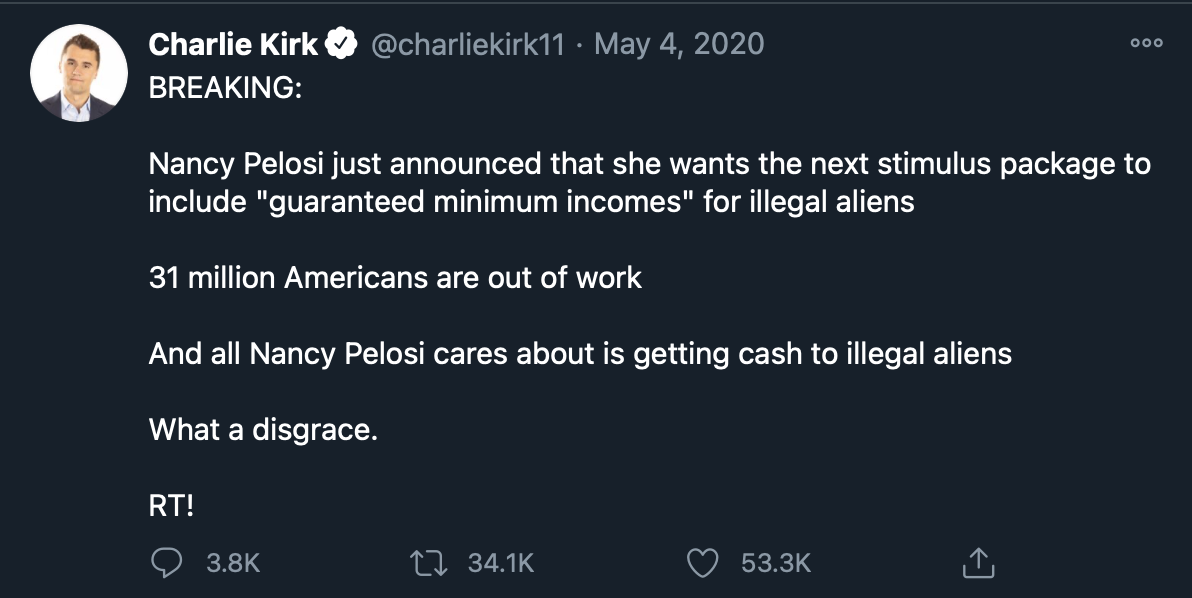
\includegraphics[width=11cm]{CharlieKirk Tweet.png}
    \caption{Charlie Kirk Tweet \cite{kirk2020tweet}}
    \label{fig:Charlie Kirk Tweet, May 4, 2020}
\end{figure} was rated ``mostly false" by Snopes \cite{lee2020pelosi}: while Speaker Pelosi did say in an interview that she wanted to \textit{consider} ``guaranteed incomes" for Americans, the rest of the tweet is not true. Therefore, since it is \textit{mostly} false but not \textit{completely} false, it would be unfair to say that $\tau_k = 0$ for this tweet; $ 0 < \tau_k < 0.5$ is more accurate. 


In another example, this tweet from Bernie Sanders is ``mostly true" (fig. \ref{fig:Bernie Sanders Tweet, Oct 13, 2020}) as most of his statements are correct, yet he leaves out that this was mostly Amazon \textbf{re-sellers} using the Amazon marketplace, not Amazon directly \cite{nicas2020sanitizer, kim2020price,gibson2020amazon}, Amazon banned over 6,000 of these price gougers \cite{bezos2020letter}, etc. Therefore, it would not be reasonable to say that $\tau_s = 1$ for this tweet; it is $ 0.5 < \tau_s < 1$. 
 \begin{figure}[h]
    \centering
    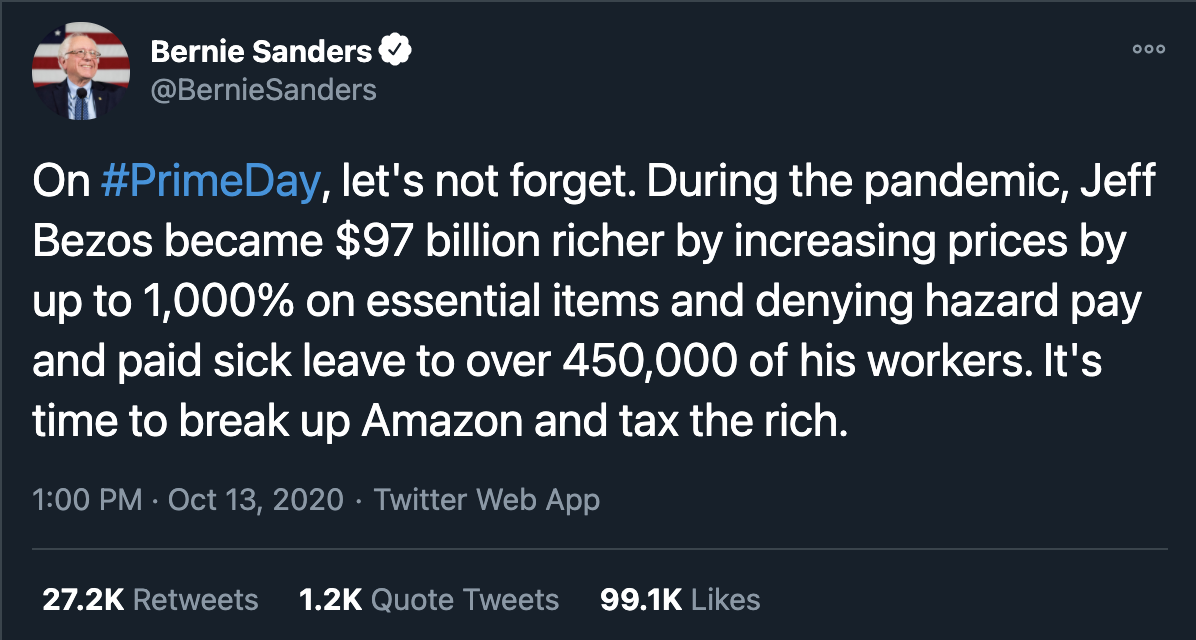
\includegraphics[width=11cm]{BernieTweet.png}
    \caption{Bernie Sanders Tweet \cite{sanders2020tweet}}
    \label{fig:Bernie Sanders Tweet, Oct 13, 2020}
\end{figure}


In \underline{Critique of Pure Reason}, Immanuel Kant proposed that statements should be broken into four groups: \textit{analytic a priori}, \textit{analytic a posteriori}, \textit{synthetic a priori}, and \textit{synthetic a posteriori} \cite{kant1908critique,frege1988collected,quine1951main}. \textit{Analytic} statements, per Kant, have the predicate contained in the subject, whereas \textit{synthetic} statements require a combination of understandings; \textit{a priori} statements are known without needing experience, whereas \textit{a posteriori} statements require experience to know if they are true \cite{wright1997companion}. For our context, table \ref{tab:misinformationexamples} provides examples of each:
\begin{table}[htbp]
    \centering
    \begin{tabular}{ |p{3cm}|p{5cm}|p{5cm}|}
    \hline
    & Analytic & Synthetic\\
    \hline
    A Priori & Hate Speech & Spam\\
    \hline
    A Posteriori &  Scientific Misinformation  & General Misinformation\\
    \hline
    \end{tabular}
    \caption{Misinformation Examples of Analytic/Synthetic Distinctions}
    \label{tab:misinformationexamples}
\end{table}
in terms of truth values, $\tau$, \textit{a priori} and \textit{analytic} statements are binary, but \textit{synthetic a posteriori} sentences may have a range of truthfulness (such as being misleading, partially true, mostly true, etc.) (table \ref{tab:truthvalues}).

\begin{table}[h!]
\centering
\begin{tabular}{ |p{3cm}|p{5cm}|p{5cm}|}
 \hline
  & Analytic & Synthetic\\
 \hline
 A Priori & $\tau \in \mathbb{B}$ & $\tau \in \mathbb{B}$\\
 \hline
 A Posteriori &  $\tau \in \mathbb{B}$  & $\tau \in \mathbb{R} \ | \ 0 \leq \tau \leq 1$ \\
 \hline
\end{tabular}
\caption{Truth Values of Analytic/Synthetic Distinctions}
\label{tab:truthvalues}
\end{table}

These proposed distinctions better capture the breadth of misinformation than the previously provided definitions: as with Klein, it concurs that intentionality is not relevant in determining truth value; unlike Wu et al. or DiFonzo \& Bordia, it makes no distinction between types of misinformation such as ``rumor" and ``misinformation"; unlike Liu \& Wu, it separates hate speech, spam, and scientific misinformation from generalized misinformation.

It is important not to separate rumor from misinformation as Wu et al. or DiFonzo \& Bordia do since rumors can be just as destructive. It also important to separate out hate speech, spam, and scientific misinformation from generalized misinformation, since there are many current machine learning solutions available for these issues \cite{xu2019exploiting,wang2010detecting,ahmed2018detecting,al2019spam,oriola2020evaluating,gaydhani2018detecting,al2020lies,farrell2019evidence}. By narrowing this thesis's scope and using these other tools in an auxiliary fashion, this thesis can focus on curbing the viral spread of misinformation that is currently being insufficiently defended against. 

\section{Literature Review}
In all of the literature reviewed for this thesis on the topic fake news, there was very little if any time spent discussing the currently implemented solutions and their shortcomings. This thesis will try to rectify that and show why alternative solutions are needed in comparison to the status quo.

In Sec. \ref{sec: literature review}, there will be a brief analysis of other relevant literature and why they fall short of solving the problem.

\subsection{Currently Implemented Solutions}
\label{sec: currently implemented solutions}
This section will look at Facebook's current solution, as it is more robust than Twitter's. Twitter currently only allows for flagging of political misinformation that is directly related to a political event, census, or impersonation.

In his 2018 testimony to congress, Mark Zuckerberg stated that Facebook's processes with content reviewers had room for improvement and then pivoted to discussing the need for AI solutions, given the high amount of content and scale-ability issues \cite{energy2018facebook}. In his 2020 testimony to congress, Zuckerberg stated that they had tripled the security team to 35,000 employees, that they're funding new security technologies to prevent emerging fake threats such as ``deep fakes", and that they have implemented resource centers for hot button topics like COVID-19 and the 2020 election \cite{zuckerberg2020}.

As of this thesis, Facebook currently has a preemptive solution and a two-step solution:
\renewcommand{\labelenumii}{\Roman{enumii}}
\begin{itemize}
\item The preemptive solution is to add a ``context” button to all political posts, which a user can click on for more information \cite{smith2018designing}.
 \item If a post has been shared and is untrue, the following two-step solution is used:
 \begin{enumerate}
     \item It requires an outside individual to report the post. 
     \item After the post is reported, then it is  sent to 3rd-party fact checkers for verification. 
     \begin{itemize}
     \item Third party fact checkers must log in to the Facebook dashboard and then provide a link proving the story is false (they cannot simply mark a story as untrue) \cite{owen2016clamping}.
     \end{itemize}
 \end{enumerate}
 \end{itemize}
 
 In Facebook’s case, after they have determined a particular post is false, then the post is shown less frequently (80 percent less), other posts of the same link or image will also be shown less, it will be unable to be converted into an ad later, and someone re-sharing this post will be given a notification that the information is likely false \cite{owen2016clamping,facebook2020fact}. The punishment for routine offenders or for routine fake stories that point to a common domain is a loss of advertising rights and a loss of ability to monetize \cite{facebook2020fact}.
 
 %%%%%% 
 \subsection{Current Literature Alternative Solutions}
 \label{sec: literature review}
 The current proposed solutions from outside published journal articles generally fall into two groupings: tools that seek to recognize all misinformation and tools that seek to recognize particular subsets of misinformation (i.e. spam).

Language analysis is, clearly, a broad subject of analysis.  Castillo et al. use a decision tree based off emojis, symbols, etc. to attempt to predict misinformation \cite{castillo2011information}. Other textual analysis includes Qazvinian's analysis of speech tags \cite{qazvinian2011rumor}, Takahashi \& Igata's examination of ``clue" words \cite{takahashi2012rumor}, Gupta et al.'s exploration of the usage of profanity \cite{gupta2014tweetcred}, Ghosh, Guo, and Muresan's investigation of word embeddings \cite{ghosh2015sarcastic}, Potomias, Siloas, and Stafylopatis's usage of a transformer \cite{potamias2020transformer}, Gaucho et al.'s review of tensor embeddings to detect content \cite{guacho2018semi}, Rubin et al.'s \cite{rubin2016fake} and Horne and Adali's \cite{horne2017just} usage of linguistic SVM classifications, Popat's investigation of how assertive verbs are in true vs. untrue content \cite{popat2017assessing}, and Riloff's \cite{riloff2013sarcasm}, Pt{\'a}{\v{c}}ek et al.'s \cite{ptavcek2014sarcasm}, Buschmeier's \cite{buschmeier2014impact}, and Barbieri's \cite{barbieri2014modelling} attempt to identify sarcasm.

For the tools that seek to recognize all misinformation, the most common solution is an RNN or an RNN/CNN combination. Ma et al. use a CNN to detect unique language patterns \cite{ma2018rumor} and Xu et al. use an RNN for the same purposes \cite{xu2019deep}, while Liu and Wu \cite{liu2018early}, Yang et al. \cite{yang2012automatic}, Wang et al. \cite{wang2018eann} Shu et al. \cite{shu2019role}, and Lee and Dernoncourt \cite{lee2016sequential}, Shu et al. \cite{shu2019beyond,shu2020leveraging} propose combination RNN/CNN solutions based off of text as well as user features (e.g. registration age) or visual clues to determine likely fake posts.  Other machine learning solutions also work off a combination of text and user information \cite{sun2013detecting,kwon2017rumor,ma2015detect,ma2016detecting,zhao2015enquiring}. VanDam uses a combination of a supervised and supervised neural network to detect hashtag and account hijacking \cite{vandam2019learning}. Chen proposes an improvement to the RNN solutions by using an attention based RNN \cite{chen2018call}. Khoo et al. also use an attention based transformer and include a hierarchical token and post level model as well \cite{khoo2020interpretable}. Zhou's SAFE model is CNN only, but it attempts to cover the same ground in a similar fashion \cite{zhou2020mathsf}.

In terms of graph analysis, Wu, Yang, and Zhu \cite{wu2015false} use a graph-kernel SVM to classify misinformation as does Ma at al. \cite{ma2017detect}. Jin et al. \cite{jin2013epidemiological} and Wu et al. \cite{wu2016mining} both identify that this problem is naturally suited to epidemiological spread. Ren et al. use a Graph Neural Network (GNN) to classify news sharing nodes \cite{ren2020adversarial} -- a similar goal to other works that focus on the user sharing the content. Hamid et al. use a GNN with a Bag of Words and BERT model \cite{hamid2020fake}, Han et al. use a GNN with continual learning \cite{han2020graph}, Rath, Morales, and Srivastava use an attention based GNN \cite{rath2021scarlet}, while Benimara et al. use a combination of semi-supervised learning and a GNN to solve the problem \cite{benamira2019semi}. Gupta et al. use a graph optimization approach \cite{gupta2012evaluating}, while others use a propagation model which tracks the cascade of content \cite{jin2016news,jin2014news,zhou2018fake,kashima2003marginalized}. Huang et al. use a combination of a GNN and a propagation model \cite{huang2019deep}. Ciampaglia et al. \cite{ciampaglia2015computational} and Shi and Weninger \cite{shi2016discriminative} use knowledge graphs and subject-predicate-object triples. Mishra et al. have used GNN's for abuse detection \cite{mishra2019abusive}, Li and Goldwasser \cite{li2019encoding} and del Tredici et al. \cite{del2019you} for political partisanship detection. Han et al. \cite{han2020graph}, Nguyen et al. \cite{nguyen2020fang}, and Chandra et al. \cite{chandra2020graph} have applied GNNs recently to the topic of fake news detection. 

 Shin et al. observe that there is a temporal relationship between rumors and truth and that misinformation can be traced to highly partisan sources \cite{shin2018diffusion}.
 
 
 \subsubsection{Issues with Preemptive Solution from \ref{sec: currently implemented solutions}}
 Facebook's proposed ``context" button (a way for users to get extra context around an article) is ineffective for several reasons. 
 
 First, it assumes that people will actively search for context when viewing a link. People are unlikely to feel the need to do further research if they agree with or believe the headline as presented \cite{nyhan2010corrections}. This problem is augmented by the fact that headlines are often misleading and written to draw the strongest possible emotional response \cite{chesney2017incongruent,ecker2014effects,bell1984good,molek2013towards,kilgo2018new,vettehen2008explaining}.  While there have been attempts to track down misleading headlines, they have primarily centered around \textit{click-bait} or tabloid headlines \cite{chen2015misleading,chakraborty2016stop} that require the user to click to find out the information. 
 
Given that only 59\% of all shared URLs are ever clicked on Twitter \cite{gabielkov2016social} and there is clear evidence of misleading headlines, Twitter added in a feature that prompts users to read articles rather than just headlines before sharing the article \cite{reuters2020article}. Unsurprisingly, the backlash was immediate: ``We tried to retweet @seanhannity’s article about @Jim\_Jordan confirming the authenticity of Hunter Biden’s emails. But Twitter slapped a warning label on the tweet before we could do it. Wow."\cite{judiciarytweet2020}.

\subsubsection{Issues With the Two-Step Solution: Echo-chambers}
\label{sec: echo-chambers}
 The key first step for the two-step solution is that an individual must report the post as false. This requires a level of self policing that it is unlikely given the prevalence of \textit{echo-chambers}. 
 
Because social media seeks to connect like minded individuals, it has a tendency to generate \textit{echo-chambers}, or closed networks with high repetition of content and low diversity of thought \cite{adibi2005proceedings, bastian2009international, pariser2011filter,bozdag2015breaking}. While not every closed homogeneous network is inherently bad -- they can operate as self-help groups \cite{kast2012under} or can encourage positive behavior like reducing prejudice \cite{paluck2011peer} -- there is a clear and well documented history that people are influenced by others in their network \cite{cialdini2004social,bollinger2012peer, bond201261,gerber2008social,gerber2009descriptive,meer2011brother,paluck2012salience,del2016spreading,bessi2015viral,friedkin1984structural,marsden1993network} and this can be destructive in the context of misinformation. For this paper's purposes, partisanship $\rho$, is defined as being on a scale of 0 to 1 with 0 being extremely left-wing and 1 being extremely right-wing (a normalized version of most one-dimensional scales of the topic). Therefore, for all users $u$ in the set of users $U$: $\forall \ u \in U \ \exists \ \rho \in \mathbb{R} \ | \ 0 \leq \rho \leq 1$.
From here, $\rho_k$, the partisan leaning of some unique user $u_k$ is directly proportional to the average partisan leaning of the \textit{echo-chamber} network $n_n$ and can be described as follows: $\langle \rho_n \rangle = \frac{1}{|n_n|}\sum_{i=1}^{|n_n|}{\rho_i}, (u_i \in n_n, n_n \in N)$, which implies $\rho_k \sim \langle \rho_n \rangle$.
 
 For validation of this, in Asch's classic experiment, he found that individuals will conform to the opinions of the rest of the group, even if it runs contrary to their personal convictions \cite{asch1956studies}. This has been proven to be especially true on political issues  \cite{bullock2007experiments,housholder2014facebook}. Even if a preferred politician's statements are disproved, there is no shift in voting intentions, party identification, or overall perceived credibility of that politician \cite{swire2017processing}. 
 
 From a network theory perspective, these two equations combine to form a version of the Hopfield attractor network \cite{hopfield1982neural,hopfield1985neural,nowak1998toward,kitts1999structural} as set forth by Macy et al.\cite{macy2003polarization}. 
 
This provides a perfect opening for malicious actors, as they are primarily focused on sharing and inflaming hyper-partisan and extreme views \cite{shin2018diffusion,bastos2019brexit,hegelich2016social,mueller2019mueller}, such that the partisanship of a malicious actor, \textit{m}, from the set of malicious actors, \textit{M}, will be extreme: $\forall \ m \in M, \exists \ \rho \in \{0,1\}$.

Mirroring viral spread seen in other scale-free network analyses \cite{pastor2001epidemic,cohen2003efficient}, this problem quickly escalates: as the number of malicious actors in the network increases, the group partisanship will shift towards the \{0,1\} binary, and given Bullock's experiments: $\forall u \in n: \rho \sim \langle \rho_n \rangle: \rho \rightarrow \rho_m$.

This equation correlates perfectly with the social experiments by Asch and Bullock mentioned previously, and more recent research has confirmed these findings \cite{colliander2019fake,edelson2011following}. Even when the groups were anonymous users on the internet, users were still be motivated by a desire to conform to the group's opinions and would, if necessary, relinquish their own previous beliefs in order to fit in \cite{williams2000cyberostracism,zhu2012switch,tsikerdekis2013effects,breitsohl2015groupthink,winter2015they,hamilton2017s}. 

The closer $\langle \rho \rangle$ gets to 0 or 1, the more closed the network becomes, and the more resistant to fact-checking or corrective information coming from outside of their network \cite{garrett2013undermining,lord1979biased,edwards1996disconfirmation,redlawsk2002hot, taber2006motivated}. This explains both why even the release of President Obama's long form birth certificate only briefly subdued the conspiracy that he was not born in the United States \cite{nyhan2012new} and why the Pizzagate conspiracy discussed in Sec. \ref{introduction} lived even after it had been disproved months earlier -- so long as the corrective information came from outside of the echo-chamber, it was fundamentally dismissed.

\subsubsection{Partisanship} 
\label{Partisanship Section}
There is substantial research that Americans who identify as right-wing have historically been more susceptible than other subsets of the American population to fake news \cite{guess2019less,benkler2018network,grinberg2019fake,allcott2017social,badawy2018analyzing}, but more thorough analysis suggests that this pattern may not hold up moving forward.

First, there may be an over representation in terms of conservative vs. left misinformation in the analyzed data sets. In the 2016 election Russian troll data set provided by Twitter that is frequently analyzed, there were twice as many right leaning trolls as left leaning trolls \cite{freelon2020black,badawy2018analyzing,benkler2018network}; however, it is likely that this is a positive feedback loop. Since conservatives were more likely to consume fake news, there were more Russian trolls creating fake content for them, which in turn these conservative users would be more likely to share \cite{bakir2018fake,bodo2019interested,silverman2016analysis,pariser2011filter}. 

Second, a better predictor of willingness to share misinformation is general distrust in the media rather than political leaning \cite{hopp2020people,shin2017partisan,kahan2012ideology,lewandowsky2016motivated,swire2017processing,mourao2019fake}. This is further born out by the Russian troll farm the Internet Research Agency (IRA) heavily targeting two groups they determined were unlikely to trust the main stream media: far right-wing Americans and Black Americans \cite{diresta2019tactics,howard2019ira,boatwright2018troll,jamieson2020cyberwar,mueller2019mueller,freelon2020black}. In fact, the IRA spent a disproportionately high amount in micro-targeting Black Americans and generated a high return on their investment \cite{howard2019ira,freelon2020black}.

Third, many sharers of misinformation are more focused on empathy with or signaling to a particular group rather than objective truth \cite{winter2015they,rheault2016measuring,dale2017nlp, connelly2011signaling,lampe2007familiar,spence2002signaling}. Dominic Cummings callously stated while creating inaccurate content for the Leave campaign for Brexit that ``accuracy is for snake-oil pussies" \cite{crace2016accuracy}, yet his point is in line with the analysis in section \ref{sec: echo-chambers}: in hyper-partisan situations, strongly held opinions that are counter to widely accepted narratives are seen primarily as signals of commonality \cite{yla2018populist,noppari2019user,lazer2018science,yla2019politicization,wasilewski2019us,freelon2020russian}. 

Fourth, there is no difference in propensity to share non-partisan misinformation, such as the dangers of living near power lines, the side-effects of MMR vaccines, or the safety of nuclear power reactors between people of various beliefs \cite{kahan2015climate,hara2016co,kahan2012ideology,lewandowsky2016motivated,barbera2015tweeting}.

Finally, most of the studies referenced previously in this section used data from 2015/2016 and before for their analysis. Since 2015, there has been a well documented global rise in populism on the left end of the spectrum to match the rise on the right that had previously existed and was documented earlier. 

This polarized shift can be statistically seen in the United States Congress by comparing the voting patterns of the 115th (Jan 2017 - Jan 2019) (fig. \ref{fig:115th House}) and 116th (Jan 2019 - Jan 2020) (fig. \ref{fig:116th House}) House of Representatives \cite{fivethirtyeight2018tracking}. In both of these illustrations, Democrats are blue, Republicans are red, Independents are orange, and the scale for each Representative is the same $0\leq \rho \leq 1$ scale seen in equation \ref{basepartisanship}. Here, a representative who always voted in line with President Trump's position (if he gave one on a particular bill) has $\rho = 1$, and someone who never voted in line with President Trump has $\rho = 0$:

 \begin{figure}[h]
\minipage{0.5\textwidth}
  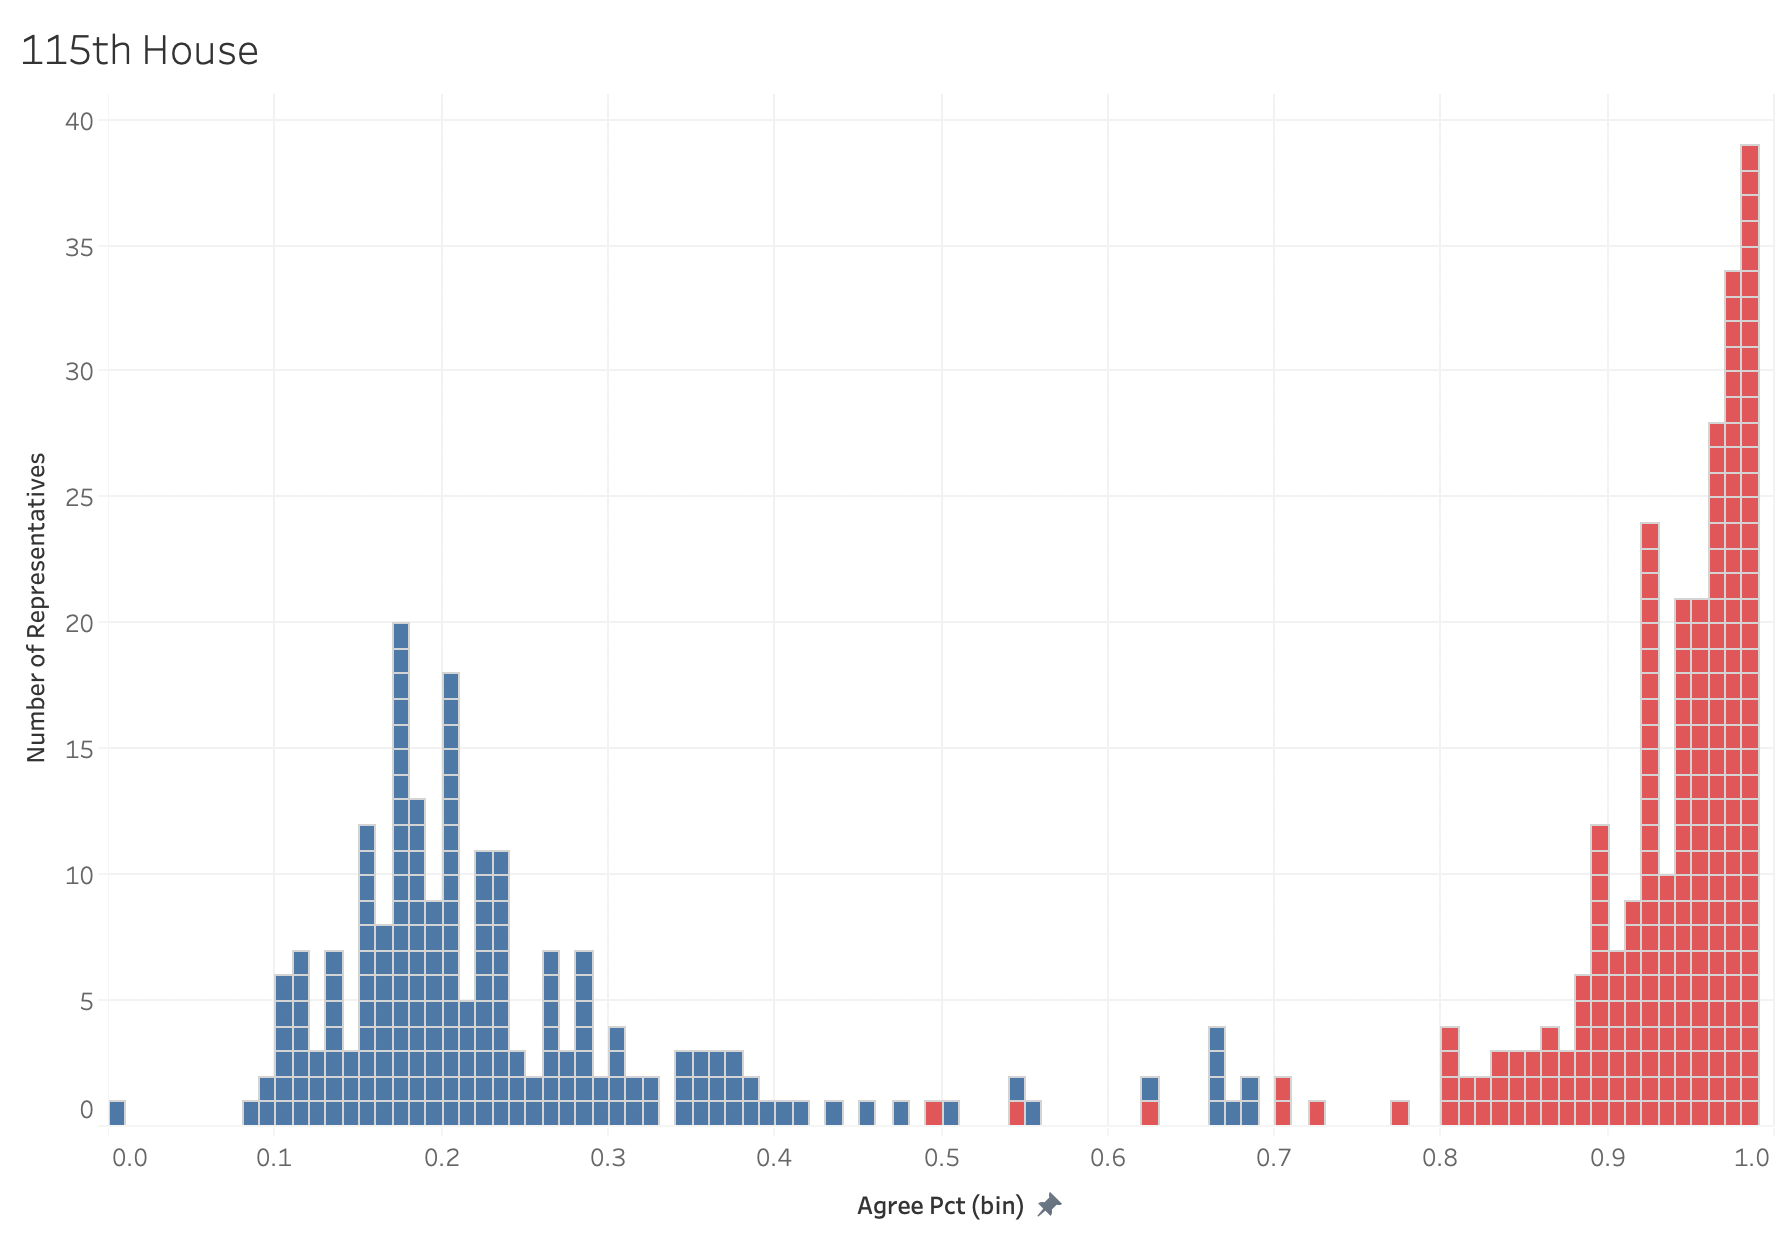
\includegraphics[width=\linewidth]{115th House.png}
  \caption{115th House of Representatives}\label{fig:115th House}
\endminipage\hfill
\minipage{0.5\textwidth}
  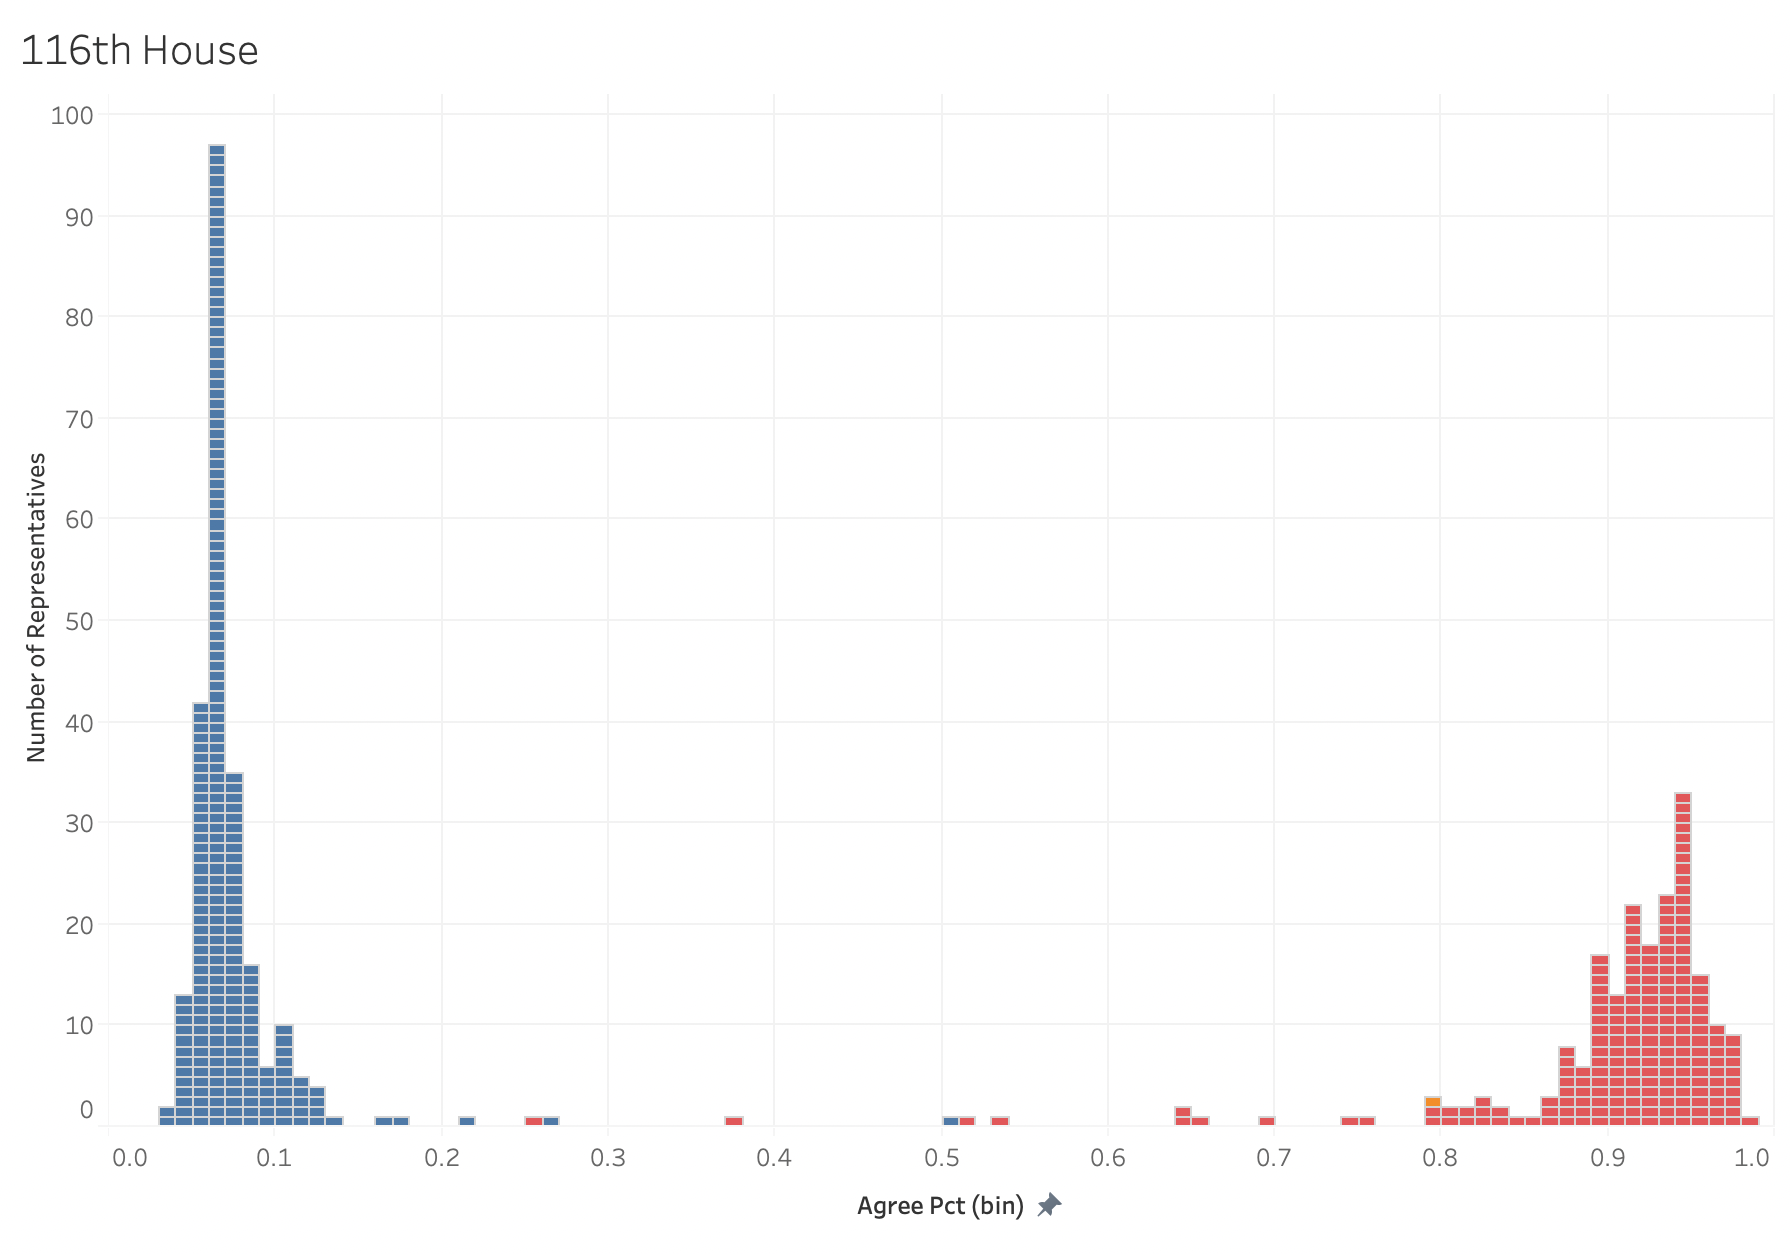
\includegraphics[width=\linewidth]{116th House.png}
  \caption{116th House of Representatives}\label{fig:116th House}
\endminipage\hfill
\end{figure}
 
 In the 115th congress, Republican members had an average $\langle \rho_r \rangle = 0.93$ and Democratic members had an average $\langle \rho_d \rangle = 0.24$. In the 116th congress, Republican members had an average $\langle \rho_r \rangle = 0.91$, Democratic members had an average $\langle \rho_d \rangle = 0.08$, and Independent members had an average $\langle \rho_i \rangle = 0.79$. For the state of Pennsylvania, which very narrowly broke for President Trump in 2016, the Democratic members had a $\langle \rho \rangle = 0.39$ in the 115th Congress and a $\langle \rho \rangle= 0.07$ in the 116th.
 
 As illustrated before, a shift in the average partisanship of the network towards the \{0,1\} binary strongly correlates to populism and a susceptibility to misinformation \cite{hopp2020people,kahan2012ideology,mourao2019fake,shin2017partisan,swire2017processing,vargo2018agenda}. This can already been seen anecdotally, as there has been an uptick in left-leaning misinformation since 2018, including information around a confrontation between MAGA-hat wearing teenagers, Black Israelites, and a Native American elder at the Lincoln Memorial in 2019 \cite{sacks2019maga,healy2019believing,pond2020complexity}, and the death of Breonna Taylor in 2020 \cite{duvall2020fact,kim2020fact}. 

 \subsubsection{Third Party Fact Checkers}
  \label{Third Party Fact Checkers Sections}
 The usage of third party fact checkers has two fundamental issues.
 
 First, there is a large volume of research over decades that ideologues on either side of the political spectrum will view identical content as being biased against them \cite{arpan2003experimental,baum2008eye,christen2002hostile,gunther2001predicting,gunther2004mapping,baum2004issue,gussin2004eye,lee2005liberal,vallone1985hostile}. This extends to fact-checking, as groups on both the left and the right post about claims of censorship when their content is removed or their reach is reduced \cite{Dreyfuss2020Now,Post2020Facebook,Millhiser2018Facebook}. 
 
 As Shin and Thorson note, however, closed networks are eager to fact check members who are not of their group. In 2018, Think Progress (a liberal Facebook fact-checker and an online journal) posted an article on the Brett Kavanaugh Supreme Court confirmation hearing that was flagged as false by The Weekly Standard (a conservative Facebook fact checker) \cite{lybrand2018kavanaugh} and by FactCheck.org, a non-partisan fact-checking organization \cite{gore2018kavanaugh}. 

Think Progress argued that secondary and tertiary definitions of ``said" made their headline correct, and instead accused Facebook of bias and censorship \cite{legum2018tweet}, ignoring that they had previously used this same yardstick to remove conservative content \cite{legum2008context, volsky2016biden, israel2018rnc, lerner2015cruz}. 
 
A better solution, clearly, would be only to use high quality non-partisan fact checkers, as they would be able to rise above the echo-chamber issues. However, these well-regarded apolitical fact checkers, such as Snopes and the Associated Press, have either left their fact checking partnership with Facebook or stopped actively working. They argue that Facebook's process is manual, time consuming, ineffective, and does not provide adequate compensation for the time required to do the job thoroughly \cite{green2019message,coldeway2019update}. 

\subsubsection{Issues with Punishment}
\label{Issues with Punishment Section}
By this point, it should be clear that the punishments imposed by Facebook are not effective, as they only seek to limit ad revenue and the ability to monetize. This implies a financial incentive for purveyors of incorrect information where, as has been shown, much of this is ideologically driven \cite{allcott2017social}. While these may be effective deterrents for the \textit{click-bait} or tabloid style headlines discussed earlier  \cite{chen2015misleading}, less than 0.1\% of traffic to fake news websites during the 2016 election came from paid media/advertising \cite{albright2016election2016}. 

The other key punishment that Facebook implements is on the actual post level. Posts deemed false are shown 80\% less frequently, and other posts showing the same link or image will also be shown less frequently. While this sounds promising, there is a fundamental flaw that can be exposed by examining Facebook's most recent papers on computer vision. Facebook's AI is a Convolutional Neural Network (CNN) \cite{carion2020end}, which is easily fooled by changing parts of the image, such as adjusting font and colors, cropping, adding filters, etc \cite{sumbaly2020using}.

Some of these had the potential to influence the 2020 election, in spite of the extra measures Facebook and Twitter added \cite{dean2020facebook}: ``While Facebook applied a contextual label to one false claim on a purple background about extra postage being required for mail-in ballots, another identical claim ran against a blue background with no intervention from Facebook. The former received 14,000 shares; the latter received 20,000" \cite{Fung2020facebook}.

\subsubsection{Scale}
\label{Scale Section}
The issue of scale is not only non-trivial, but is unmentioned in the other literature on solving this issue. Attempting to crawl through every tweet and every URL posted would be an incredibly difficult task given that Facebook alone has 1.8 billion daily active users according to their Q3 2020 earnings report, with 2.54 billion daily active users of at least one tool in the Facebook portfolio (Facebook, Instagram, WhatsApp, etc.), with those numbers ballooning to 2.74 and 3.21 billion on a monthly level \cite{facebook2020q3}. Given that in 2014 Facebook generated 4 petabytes of data daily and ran 600,000 queries with 1 million map-reducing jobs when their total daily active users was 890 million \cite{bronson2015open}, a simple ratio would provide a conservative estimate that Facebook now generates at least 8.1 petabytes of data every day, with 1.2 million queries and 2.1 million map-reducing jobs. 

Many of the proposed solutions for fake news detection are RNN based, however RNNs are far too resource heavy to be successfully implemented at the necessary scale \cite{gehring2017novel, sze2017efficient}. Even transformer based attention models require high amounts of computational power and primarily excel at tasks like language translation \cite{vaswani2017attention}. 

As Liu points out in their 2019 thesis \cite{liu2019early}, each RNN is topic specific. Because of that, it begins with 0 information when the misinformation topic begins and requires a great deal of time to build up enough of a base to be successfully trained and deployed. In some crisis situations, that time may not be available. This criticism holds true for the propagation models as they require too much time before they can be successfully deployed.

The GNNs mentioned in the literature review section similarly struggle with scale. Han et al.'s GNN, for example, only looks at surface level user data such as length of user name; Chandra et al.'s GNN looks at who is consistently sharing misinformation, but it is topic specific as well and requires an extensive history of historical misinformation sharing; Nguyen et al's GNN creates only two homogeneous graphs - one looking at news sources and one looking at users - which misses the clear connections between the patient zeroes and the spread of a disease.

Every single neural network discussed here is therefore ``hack-able" at the point that malicious actors determine the pattern being used to allocate a post into a remove/don't-remove bucket. Several of these neural networks include surface level data like length of user name -- if a malicious actor discovers that their disinformation is being flagged simply based off of user name length, all they have to do is change their user name and their content is allowed to flow freely. This would require every one of these neural networks to be re-trained on an iterative basis, which is unsustainable.

\subsubsection{Hyperbole, Sarcasm, and Irony}
\label{hyperbole}
Current literature using NLP to decipher sarcasm and irony primarily revolves around unexpected word combinations \cite{barbieri2014modelling,buschmeier2014impact,ghosh2015sarcastic} or RoBERTa recurrent neural networks \cite{potamias2020transformer}. Many of these are able to generate quite high F1 scores; however, as Oprea and Magdy point out, tools that are successful in one data set struggle in other data sets. Models trained in the Riloff data set can generate an F1 score above 0.8, but those same models will generate an F1 score near 0.5 (which is the same as random guessing) when applied to the Pt{\'a}{\v{c}}ek set \cite{oprea2019exploring}. This implies there are extreme differences in how groups express and perceive irony/sarcasm/hyperbole. Those differences are beyond the scope of what RNNs and RCNNs can currently successfully grasp. Therefore an alternative solution to handling irony on a global level is necessary. 
 
\subsection{Alternative Solution: Flatten the Curve}
\label{Flatten the Curve Section}
Forcing $\tau$ into a binary does a disservice to everyone involved. As discussed when comparing Bernie Sanders's tweet (fig. \ref{fig:Bernie Sanders Tweet, Oct 13, 2020}) and  Charlie Kirk's tweet (fig. \ref{fig:Charlie Kirk Tweet, May 4, 2020}), neither of those statements should have a truth value equal to 0 or 1, but neither should their truth values be equal to each other. Therefore any kind of \{0, 1\} regression or classification is fruitless and ultimately working in the wrong direction. Similarly, as illustrated in \ref{hyperbole}, there are currently no solutions that show similar results when tested on completely unique data sets of irony/hyperbole/sarcasm. Therefore, there is a high probability that ironic, hyperbolic, and sarcastic tweets would also be set to $\tau = 0$ and be flagged for removal, when they should not be. Machine learning is not the right tool to solve this problem. 
 
 Instead, this thesis proposes an alternative way of viewing this problem: a virus that needs to be curbed. The similarities are clear and even baked into our own language on the topic -- when a social media post spreads rapidly, it's called ``viral". 
 
 By examining misinformation as an epidemic, the focus shifts from a classification problem, to aiding the doctors that can diagnose and resolve the disease: the fact-checkers. In \ref{Third Party Fact Checkers Sections}, evidence was presented that high quality fact-checkers are leaving because the platform is too cumbersome. There are simply too many posts to comb through, they have to keep rechecking identical posts, and they are not paid commensurate with the time required to do the work. While Zuckerberg proposed to use AI to handle the misinformation categorization, a better solution is to view this as an optimization problem: how can a fact checker's time be maximized? 
 
 \subsubsection{Universal Fact-Checking vs. Proportional Fact-Checking vs. Targeted Fact-Checking}
 The current solution works as a de-facto universal fact-checking: there is no threshold that must be met before the two-step solution is implemented. The machine learning solutions discussed in \ref{sec: literature review} also propose a universal ``always on" fact checking solution. In analysis of viral spread, this universal fact checking is akin to ``uniform immunization", where immunized individuals are entered into the population. This solution is completely ineffective as it reduces the spread of the disease too slowly, and it is impossible to determine a minimum fraction of individuals who need to be immunized in order to ensure that the infection dies off, unless every single individual becomes immunized \cite{pastor2002epidemic,pastor2002immunization,anderson1992infectious}. In order for a uniform fact-check to work, upwards of 80\% of all tweets would have to be fact-checked \cite{may1984spatial,hethcote2014gonorrhea,hethcote2013modeling,hethcote1987epidemiological,albert2000error, pastor2001epidemic}, as a network can remain contagious even after the majority of nodes are removed \cite{cohen2000resilience}. Indeed, in this context, the fraction of users $v_c$ that would need to be immunized/vaccinated and removed in order to make the network no longer contagious, $v_c \rightarrow 1$ \cite{cohen2003efficient,strogatz2001exploring,albert2002statistical,dorogovtsev2002evolution,pastor2002immunization}.
 This means that all tweets would have to pass through a fact-checking process before they could be made live, which is an impossibility at current scale and would completely destroy the business model of social networks (section \ref{Scale Section}).
 
 An alternative solution may be a proportional fact-check, where the fraction of tweets to be fact checked is proportional to their relevance in the network. For example, since there were twice as many right leaning trolls as left leaning trolls in the IRA data set \cite{freelon2020black,badawy2018analyzing,benkler2018network}, conservative content should be checked twice as frequently; however, it too runs into myriad problems. First, it does not resolve the issue of fact-checkers having to sift through unimportant content. In a 2018 analysis of over 700 million tweets, Mention discovered that while the mean number of retweets is 1,696, the median is 0 \citep{mention2018twitter}. By proportionally allocating attention based off of partisanship, fact checkers will end up spending a great deal of time confirming or disproving content that nobody will likely see. This is akin to sending epidemiologists to vaccinate hermits and ignoring the metropolis. 

Second, while proportional immunization is more effective than uniform immunization, it is not the most efficient solution \cite{dezsHo2002halting,anderson1992infectious}. The fraction needed to immunize, $v_c \approx \lambda^2/3 $, where $\lambda$ is the rate of spread of a disease \cite{pastor2002immunization,barabasi1999emergence}. This is better than $v_c \rightarrow 1$, but not ideal. Networks are incredibly resistant to the loss of random nodes and are able to recover quickly \cite{cohen2001breakdown,callaway2000network,albert2000error}.

Instead, an ideal solution must be targeted in approach.
 
 
 
 \subsubsection{Proposed Solution}
 \label{sec: proposed solution}
 
 As just discussed, not all users are equally important, nor are all posts are equally important. As Grinberg et al. confirmed, only 1\% of users accounted for 80\% of the total exposures to fake news posts in the 2016 election and only 0.1\% of users (approximately 57,000) accounted for 80\% of the total shares of fake news posts in the 2016 election \cite{grinberg2019fake}. 29 million people follow only 10 individuals who are the biggest purveyors of anti-vaccine content \cite{npr2021teachers,ahmed2020antivaxx}. Removing these 10 individuals would dramatically cripple the anti-vaccine movement.
 
 The ideal solution, then, is to treat this is a ranking problem. Many other applications of network theory that focus on immunizations also illustrate that the removal of just a fraction of the total nodes can cause the entire network to disintegrate \textit{if} those nodes are intentionally and correctly selected  \cite{albert2000error,callaway2000network,cohen2003efficient,helleringer2007sexual,cohen2001breakdown,hethcote2014gonorrhea,cohen2000resilience}.
 
 For the set of tweets that must be fact-checked, $F \subset T$, we can create an ordered set $F^*$ such that $F^* = (t^*, t_1, t_2 \cdots t_n), \ t^* \succ t_1 \succ t_2 \cdots \succ t_n$. To determine the ranking, let $\mu \in \mathcal{M} | \mathcal{M} \in \mathbb{R}$ be the set of relevant numerical metrics available for each user/tweet combination and $\beta \in B| B \in \mathbb{R}$ be the set of unique weights per metric. These can be summed: $\zeta = \sum_{n=0}^{|A|} \beta_{n} \cdot \mu_{n}$, meaning for tweets $t_i$ and $t_j$: $\zeta_i > \zeta_j \Rightarrow t_i \succ t_j : t_i, t_j \in F$.
 
  This allows for the fact that there will always be more posts that need to be checked than can be physically checked in a day, but also ensures that the most dangerous -- the ``super-spreaders" -- are stopped first.
  


\section{Network Theory}
For these sets, the language will be that of Twitter (tweets, following, hashtags, etc.) yet the terms are easily translated to other social media groups such as Facebook, Instagram, etc.

First, for any user in the set of all users, such that $u_n \in U$, there exists a ``network", $n_n \in N$ which consists of all the other users that $u_n$ follows or is followed by. This can be further parsed out into $Y_n$, the set of users who follow this user, and $Z_n$, the set of users who are followed by this user:  $N_n = Y_n \cup Z_n$. 

Typically, the number of connections in the network $k_n$, is $k_n = |N_n|$. $k$ is directionally agnostic, such that $k_{ij} \equiv k_{ji}$. For this analysis, however, directionality is important: if $u_i$ followers $u_j$, there is no implication of a reciprocal relationship. Therefore, since directionality is important, this thesis will use $\Psi_n$, where $\psi_{ij}$ represents user $i$ following user $j$: $\psi_{ij} \in \Psi, u_j \in Z_i: i \neq j$ and $\psi_{ji} \in \Psi, u_j \in Y_i: i \neq j$. However, this thesis is primarily focused with how many users follow a particular user, not how many users they follow. Therefore, unless otherwise stated, let $\psi$ \textbf{only} represent inbound connections such that $\psi_{ji} \in \Psi, u_j \in Y_i: i \neq j$.
    

\subsection{Background on Networks}
\label{sec: Background on Networks}
This thesis will focus on Facebook and Twitter, both of which are \textit{scale-free networks} \cite{aparicio2015model,broido2019scale,barabasi2000scale} since they are networks with very few well connected nodes, called hubs, and mostly unconnected nodes \cite{barabasi2009scale,barabasi1999emergence,dorogovtsev2002evolution}. The probability of one node (here a user, \textit{u}) being connected to some large number of other users, $k$, in comparison to the average number of connections, $\langle k \rangle$, is $P(k) \sim k^{-\gamma}, 2 < \gamma \leq 3$
In comparison, small networks tend to have uniform distribution of \textit{k}, such that $k \cong \langle k \rangle$: in other words, everyone is friends with everyone \cite{erdHos1960evolution,watts1998collective}.

Aparicio, et al. confirmed that Twitter followed the power-law distribution and found that for an average user $U_n \subset U:\langle | Y_n| \rangle \leq 100, \langle | Z_n| \rangle \leq 1,000$. This very low ratio of in to out tracks with other research on networks which show that an individual's contacts are likely to be more connected than they are. This observation spans social networks such as friendship, computer virus spread, STD transmission, etc. \cite{feld1991your,newman2003ego,pastor2001epidemic,pastor2002epidemic,pastor2015epidemic,helleringer2007sexual,hethcote2014gonorrhea,liljeros2001web}.

On the other hand, for hub nodes $U_h \subset U: \langle | Y_h| \rangle = 67,622, \langle | Z_h| \rangle = 47,351$. This hub sub-network was generated by minimizing the number of edges to connect all nodes with each other, which created a subset of only 0.002\% of the total set of users. This is in line with the Barab{\'a}si-Albert's preferential attachment equation, with the probability, $P(\cdot)$, that a new node to the network connects to node $i$ depends on the degree $k_i$, where $j$ are all the other pre-existing nodes:
\begin{equation}
\label{preferentialequation}
    P(i)=\frac{k_i}{\sum_{j} k_j}
\end{equation}
since $\sum_{j} k_j$ is constant for any network at the instant of a node's choice, the likelihood, $L(\cdot)$, that a node new to the network chooses to connect to unique node $i$ over unique node $j$ is (with $a \succ b$ representing that $a$ is preferable to $b$) :
\begin{equation}
\label{likelihood equation}
    L(i \succ j)=\frac{P(k_i)}{P(k_j)} = \frac{k_i}{k_j}
\end{equation}

\subsection{Proposed Adjustments to P($\cdot$) and L($\cdot$)}
As of yet, no literature has attempted to combine the Barab{\'a}si-Albert preferential equation, equation \ref{preferentialequation}, with the partisanship analysis performed in \ref{Partisanship Section}.

Let the null hypothesis $H_0$ be that partisanship has no bearing on the preferential attachment equation, and let $H_\alpha$ be that it does, so that for user $u_n$ deciding between two other users $u_i$ and $u_j$, $\rho_{\Delta}$ will be the absolute value of the difference between these two partisanships (i.e. $\rho_{\Delta} \in \mathbb{R} \ |\  0 \leq \rho_{\Delta} \leq 1$, where 0 means complete agreement and 1 means complete disagreement). Including $\rho_\Delta$ into equation
\ref{likelihood equation}:
\begin{equation}
\label{Ldotpartisan}
        \tilde{L}(i \succ j)=\frac{k_i(1-\rho_{\Delta_i})}{k_j(1-\rho_{\Delta_j})},\rho_{\Delta_j}\neq 1 
\end{equation}

If $\rho_{\Delta_j} = 1$, then it should be self evident that $i \succ j$, regardless of $i$'s partisanship; if $\rho_{\Delta_i} = 1$ \textit{and} $\rho_{\Delta_j} = 1$, then the user is stuck between two unpalatable solutions and is as likely to pick either of them as to pick neither. By extension, if equation \ref{Ldotpartisan} is accepted, then an adjustment to P($\cdot$) is necessary as well:
\begin{equation}
\label{Pdotpartisan}
        \tilde{P}(i)= \frac{k_i(1-\rho_{\Delta})}{\langle k \rangle  (1-\langle\rho_{\Delta}\rangle) }
\end{equation}
Both of these equations are logical converses to the accepted Hopfield equation discussed earlier. While Macy et al. move from this equation to an examination of the probability that a user will change their mind based on the social pressure surrounding a particular topic so as to maintain a social balance and minimize dissonance \cite{macy2003polarization}, it also logically follows -- building on the same works \cite{kitts1999structural,heider1982psychology,cartwright1956structural,hopfield1982neural,hopfield1985neural,nowak1998toward} -- that a person in balance will seek to stay in balance as they add nodes to their network. In other words: partisan inertia.

If $\langle \rho_{\Delta} \rangle$ is unknown, as is a likely scenario, it can be set to 0.5. This is because $1 - \rho_{\Delta}$ effectively measures the distance in partisanship away from the center, which would make an average set of neutral content $ 1 - \langle\rho_{\Delta} \rangle = 0.5$. As Mosley, Martel, Eckles, and Rand confirmed, when presented with two potential connections with equal $|\psi|$ values, individuals will select the connection that matches their partisanship over a neutral one. They found ``evidence of a positive three-way interaction between co-partisanship, bot partisanship strength, and user partisanship strength" \cite{mosleh2020shared}, with no difference between highly partisan Democrat and highly partisan Republican activity. 

At the same time, by using the average partisanship spread of the network (when known), the results are more precise and can come into better focus. They also help explain the ``unlikely ally" in ``enemy territory" scenario: someone with $\rho = 0$ in a community of $\langle \rho \rangle=1$ will prefer to connect with a $\rho = 0.75$ if they are the closest possible value, even though they might never connect with a $\rho = 0.75$ in any other situation. 

This hypothesis breaks down into two sub-hypotheses: \\
\textbf{$H_1$}: There is a statistically relevant relationship between followers and partisanship, such that more extreme partisanship is rewarded with more followers \\
\textbf{$H_2$}: There is a statistically relevant relationship between the members of the set of followers and the partisanship of the user.

 \subsubsection{$H_1$ and $H_2$}
 \label{H_1 and H_2}
 To test $H_1$ the Twitter follower count of each representative in the 116th congress was attached to their voting records by accessing the Twitter API using the \textit{Tweepy} library. For representatives with multiple accounts, the account with the higher number of followers was selected and representatives without a Twitter account were removed from the data set. 

A $\chi^2$ test was then performed on the Republican representatives ($n = 199$) resulting in a the $p$-value for this test was $p=0.0005$. Therefore we can say that the null hypothesis should be rejected, and we should conclude that there is a relationship between twitter followers and voting patterns.

To test $H_2$, two members of the 116th house with similar twitter follower sizes were selected: Rep. Devin Nunes, who had 1,272,026 followers as of 1/10/20, and voted in line with Trump 93\% of the time and Rep. Rashida Tlaib, who had 1,332,772 followers as of 1/10/20, and voted in line with Trump 12\% of the time. From a random set of 5,000 followers of each representative (which would give an $\alpha = 0.01$ and a confidence interval of $\pm 1.8\%$), the similarity socre was 0.28\%. In comparison, Rep. Kevin McCarthy, who voted with the President 95\% of the time and has 1,175,068 followers, had an 11\% similarity score to Devin Nunes.

This experiment was repeated with the top 5 members of each party of the 116th congress by twitter followers: Democrats Lewis, Pelosi, Ocasio-Cortez, Tlaib, and Omar; Republicans Nunes, McCarthy, Jordan, Gaetz, and Crenshaw: this resulted in a net resulted 1.08\% similarity score.

Given the low Jaccard indices for cross-party followers and a higher intra-party index, we must reject the null hypothesis that there is no correlation between party affiliation and follower similarity scores. Indeed, \textbf{there is at least 8x more overlap in followers of the same party than across parties, yet on an individual level this rate is closer to 40x}. 

Since both $H_1$ and $H_2$ are accepted, the proposed adjustments to $L(\cdot)$ and $P(\cdot)$, equations \ref{Ldotpartisan} and \ref{Pdotpartisan}, are accepted.

\subsection{Proposed Adjustment to the Average Partisanship Equation}
As shown in equation \ref{Ldotpartisan}, there is a correlation between partisanship and similarities in the sets of followers, validating the hypothesis of the existence of echo-chambers. However, it also illustrates that a new user will find $u_i \succ u_j$ based off the combination of relative partisanship and current followers. This combination provides:$\langle \rho_n \rangle = \sum_{i=1}^{|n_n|}\rho_ik_i / \sum_{j}k_j | \ u_i \in n_n, n_n \in N$.


\section{Metrics For Ranking Function}
\subsection{Four Proposed Metrics}
This thesis proposes that the seven W's (``Who", ``What", ``Where", ``When", ``Why", ``How", and ``With What") that come from Aristotle \cite{sloan2010aristotle,aquinas1952thomas} be the basis of this thesis. Of these seven, three are self-evident or irrelevant: the ``where" is social media; the ``by what means" and the ``why" are not relevant to our examination. Therefore, this thesis narrows these questions down to four: Who is sharing the content, what are they sharing, how quickly is it spreading, and how far along is it?

\subsection{Who is Sharing?}
At first glance, the ideal solution is simply to focus on the hub nodes, however this requires a great deal of, if not complete, knowledge about the network in advance  \cite{dezsHo2002halting,pastor2002immunization}. That having been said, since social media users have $|Y|$ values readily available, this still seems to be an easy solution. However, the $|Y|$ value of a ``hub node" is an inconsistent metric - at its peak, @TEN\_GOP had around 100,000 followers, but other troll accounts identified in the Mueller report had lower $|Y|$ values:

\begin{quote}
Individualized accounts used to influence the U.S. presidential election included @TEN$\_$GOP (described above); @jenn$\_$abrams (claiming to be a Virginian Trump supporter with 70,000 followers); @Pamela$\_$Moore13 (claiming to be a Texan Trump supporter with 70,000
followers); and @America$\_$1st$\_$ (an anti-immigration persona with 24,000 followers). \cite{mueller2019mueller}
\end{quote}

Based on a broad analysis of twitter as a whole, (and the average metrics provided by Aparicio et al. \cite{aparicio2015model}), the average $|Y|$ value for a hub node is 67,622. This would catch some of the troll accounts listed but not all of them. Nor would it catch Facebook groups with low numbers of highly active people: unarguably, a group with a small number of people who are constantly active is more worthy of attention than a large group where nobody is active.

This may seem like an impossible ball to untangle at first, but equations \ref{ech chamber}, \ref{peopletoextremes}, and \ref{echo-chamber by followers}, illustrate that an individual's partisanship is directly related to the partisanship of the most connected person in their network. While one might argue that an individual might follow opposing view points, the analysis in section \ref{H_1 and H_2} shows that this is statistically unlikely to be the case. Similarly, one might argue that merely following someone does not necessarily imply $\rho_i \simeq \rho^*$, where $i$ is the unique user and $\rho^*$ is the partisanship for $u^*$, the user with the $\max(|\psi|), u^* \in Z_i$. This thesis does not deny that. However, users who follow $u^*$ are likely to follow other similar users with similar viewpoints (eq. \ref{Ldotpartisan}), and the probability that an individual follows a user who shares misinformation is not changed by the individual's reaction to the misinformation (eq. \ref{probability of infected node}).

Let $\vec{A_i}$ be a vector of ordered pairs of all users that $u_i$ follows and their corresponding follower counts: $\vec{A_i}=\{(u_1,|\psi_1|),(u_2,|\psi_2|),(u_3,|\psi_3|)\dots (u_n,|\psi_n|)\}, u \in Z_i, \psi \in \Psi$.

By all the equations and background discussed earlier, the most important $u \in Z$ is the user with corresponding $\max(|\psi|)$. This allows for private groups, reportedly a key place where the riot at the U.S. Capitol on January 6th was planned and misinformation was spread \cite{yin2021facebook,horwitz2020facebook}, to be included: $|\psi|$ for said group is the number of members who belong to it. Let $U^*$ then be the set of all users who are a $u^*$ for at least one other user.

We can then determine the number of times a particular user appears in that set, which will be the first metric: 
\begin{equation}
\label{mu_1 equation}
    \mu_1 = \sum_{u\ \in \ U^*}1_{\{u_i\}}(u)
\end{equation}

This proposed equation operates as a more refined version of Cohen et al.'s strategy for immunization \cite{cohen2003efficient}, which is effective with ecological networks \cite{sole2001complexity,camacho2002robust}, metabolic networks \cite{jeong2000large}, cellular proteins \cite{jeong2001lethality}, and terrorist networks \cite{cohen2003efficient}. 

\subsubsection{White Listing}
\label{sec: white listing}
Some users with a very high $|\psi|$ value are known news outlets, comedians, sports organizations, etc. which do not require the same level of scrutiny that other accounts do. This list can have an established cadence for review, so that athletes or journalists who begin tweeting misinformation (as in the cases of actor Woody Harrelson, UK boxer Amir Khan, and US rapper Wiz Khalifa tweeting about 5G causing COVID \cite{bruns2020covid19}), can have their white-listed privileges revoked. 

If a user is in this set of white listed users, then they would be removed from $\vec{A}$ for all users, thus preventing from being considered a $u^*$.

\subsection{What is Being Shared?}
\label{sec: what is being shared}
Currently, Twitter, Facebook, and other social media companies label topics as \textit{trending}, which is based almost exclusively on kurtosis over a very small window of time \cite{dewey2015freddie,lotan2015freddie}. 

When the elapsed time from a post's creation to the moment of inspection, $j$, is sufficiently small, it's possible to draw incorrect conclusions about the actual velocity of the content. Trending, per Lotan \cite{lotan2015freddie}, operates more akin to jerk in physics and is connected to the the number of retweets at the moment: $\partial^3 r / \partial j^3$.

There are two flaws here. First, using $r$ favors topics that may or may not quickly expire on their own while ignoring slowly growing topics. In the Washington Post article cited earlier, \#FreddieGray was never considered trending on Twitter even though the story was featured prominently on CNN, ABC, the New York Times, etc. and more than 150,000 people tweeted on the topic on April 25, 2015.

Sociologist Zeynep Tufekci argues in multiple media that this becomes de-facto censorship \cite{tufekci2017twitter,tufecki2018democracy,tufekci2017we,tufekci2014online}. She provides numerous examples, such as Facebook's 2014 trending window which provided high visibility to topics such as the ``Ice Bucket Challenge", but completely left off the protests in Ferguson, MO after the shooting of Michael Brown. This, she contends, creates effective censorship: by denying visibility to a particular topic while elevating another, social media is making (whether intentional or not) editorial decisions. 

\subsubsection{Current Literature Alternatives} 
Because social media posts are filled with spelling errors, typos, abbreviations, lexical variations, etc., it is incredibly difficult to gather a precise understanding of the post in a reasonable amount of time \cite{vandam2019learning,laniado2010making,schubert2014signitrend}. Dashtipour et al. analyze how reliant text analysis is on a robust lexicon, which will always lag behind common usage of language, and some languages have more thorough lexicons than others \cite{dashtipour2016multilingual}.

VanDam, however, proposes a neural network that runs on the set of each unique user's tweets (rather than a global dictionary) to detect if a post is ``out of place", which can point towards a compromised account, or if a hashtag has been ``hijacked" and users are sharing unrelated or negative content with the hastag attached  \cite{vandam2019learning, vandam2016detecting}. While this solution is useful, it only detect outliers against a pattern. In examples where the hashtag is primarily being used as a beacon of disinformation, such as \#stopthesteal and \#sharpiegate during the 2020 election to signal election fraud \cite{perez2020facebook}, this solution would be ineffective.

Another way to determine topic importance is to use top-k modeling \cite{babcock2003distributed}, but this solution measures \textit{volume} and not \textit{importance}, which is not a relevant metric for this thesis. 

\subsubsection{Word Pair Hashing}
This approach to content analysis borrows heavily from the insights of Schubert, Weiler, and Kriegel, who also observed that current solutions, such as TF-IDF or First Story Detection (a model to detect the first reporting of an incident \cite{petrovic2010streaming,yang1998study}), require a great deal of memory. They detected that this scaling issue gets even worse when looking at word pairs -- an alternative solution, \textit{enBlogue}, retains $2p$ historical values for any word pair, with $p$ being the number of recent occurrences of the pair \cite{alvanaki2012see} -- which leads to retaining data for at least 700 million word pairs at any given point in time \cite{schubert2014signitrend}. Given all of the unintentional and intentional issues with social media posting spelling and grammar, that number has the potential to balloon significantly. 

Instead, Schubert, Weiler, and Kriegel propose a word pair hashing system with a half-life. This half-life inclusion allows for word pairs to be removed from the set as they cease to be relevant, thus freeing up memory, but also allows for topics that grow at a slower rate not to get lost in the shuffle. Furthermore, by hashing the words, the system has no need to store any lexicographic information -- it also resolves the issues presented by Dashtipour et al.

They propose a model based off of the Exponential Weighted Moving Average (EWMA) and variance (EWMVar). By using moving average and moving average variance, this prevents topics that had a very high amount of discussion a long time ago from retaining any supremacy. 

They tested their solution on posts about Edward Snowden's flight from Hong Kong to Moscow. At that time, posts about Snowden were already quite prevalent, so the words \textit{Edward} and \textit{Snowden} had started to drop off from their ``trending" metric due to a lack of novelty, but various combinations of the word set \{\textit{edward, snowden, hong, kong, moscow}\} exhibited significant peak. 

\subsubsection{Process}
The daily process and analysis would be in two parts: indexing and analyzing.

For indexing, every document will have each word pair indexed in the hash table, such that its moving average and moving variances are recorded and updated as more frequencies of the word pairs appear. At each point, as a final step of the indexing process, the frequency of that word is measured against a maximum $z$-score ($\beta$ here is a constant to ensure that the denominator is not zero): $z = \frac{x-\max\{\mu, \beta\}}{\sigma + \beta}$. If that $z$ exceeds the threshold for alerting, then it is immediately routed to an early alert system.

For end-of-day analyzing, both the EWMA and EWMVar tables are updated such that words with lower popularity are overwritten with new pairs with higher popularity. Terms are also analyzed for their $z$-score as calculated above here, which provides a list of terms that trended that day. Those terms are both worthy of further investigation and are potentially a warning for what will trend tomorrow.

\subsubsection{Summary}
\label{what is being shared summary}
When analyzing Twitter data utilizing a streaming API over 114 days, this process captured 279 million tweets -- approximately 1\% of all tweets during that period -- which turned into 6.7GB of processed data. Processing this twitter data took, on average, 46 seconds per day; the actual analysis took, on average, 25 seconds per day; the data storage required, on average, was only 160MB per day.Clearly, this process can be applied to the full Twitter ``firehose" without issue and without need for further adjustments.

Furthermore, this solution solves the problem posed at the beginning of this section where important topics with small kurtosis were drowned out and went unnoticed. Since the key words are held in tables and moving averages are used, topics with high trending but low sustainability (such as a sports event or TV event) will enter and leave the tables quickly, while topics that show low but consistent growth (such as \#FreddieGray) will remain present. 

Therefore, let $I$ be the set of trending topics as determined by the tables described previously with $i$ being a unique pair, $z$ be the $z$-score result generated from the exponential moving average/variance tables, $s$ be the significance level, and $d$ be the number of days (not necessarily consecutive) that this topic has been in the tables .

This provides $\mu_2$ which can give us the importance of the content being discussed:
\begin{equation}
\label{mu_2 equation}
    \mu_2 = \begin{cases}
    z\cdot d  & \text{if}\ i \in I\ \text{and}\  z > s \\
    0\  & \text{if}\ i \notin I \ \text{or} \ z \leq s
    \end{cases}
\end{equation}

As a final note here, it is worth mentioning that none of the previously discussed neural networks accounted for the fact that they would need to be perpetually trained to be effective. As seen here, moving averages are important: topics that were important yesterday are not necessarily important today. Patterns of fake news yesterday that have been identified can be easily changed to create fake news today. This is yet another flaw to the proposed self-sustaining neural network solutions.

\subsection{How Fast is it Spreading?}
\subsubsection{Standard Rate of Transmission: $\lambda$ Value}
There are many ways to determine transmission rate, $\lambda$. For this thesis, $\lambda$ will be the derivative of the cumulative sum of retweets. 

While users will unquestionably read content without retweeting it, Gabielkov et al. observed that the relationship between retweets and total followers can be used to project times that a user has seen content without sharing it \cite{gabielkov2016social}.

Therefore, let $y_j$ be the cumulative sum function $y_j = \sum_{i=o}^j r_i$ where $r_i$ is the number of retweets at that particular point in time. $y_j$ can be further understood to be a natural log function of time, based on analysis of retweet paths over time \cite{gabielkov2016social,starbird2014rumors,mention2018twitter}, such that for any tweet, the total retweets over time maps to $f(j) = a \ln j$, where $a$ is a constant. This means that the rate of change: $f'(j) = a /j = \lambda$

\subsubsection{Standard Critical Rate of Transmission: $\lambda_c$}

Given the density equation for infected nodes $d \sim \exp( - C / \lambda)$ where $C$ is a constant and $\lambda$ is the rate of transmission \cite{pastor2001epidemic}, the equation for $\lambda$ can be merged in to provide: $d \sim \exp((-C j)/ a)$.

The dynamic mean-field reaction rate \cite{marro2005nonequilibrium,pastor2001dynamics,pastor2001epidemic} as relates to $j$ for a node with $k$ connections (here $d_k(j)$ is the relative density of nodes with $k$ connections) is: $\partial_jd_k(j) = - d_k(j) + \lambda k \big(1 - d_k(j)\big)\Theta(\lambda)$. At this point, let $\psi$ be substituted in for $k$, as with the previous equations: $\partial_jd_{\psi}(j) = - d_{\psi}(j) + \lambda \psi \big(1 - d_{\psi}(j)\big)\Theta(\lambda)$.

By setting the mean field equation to a static state ($\partial_jd_{\psi}(j) = 0$), the $d_{\psi}$ can be solved for: $d_{\psi} = (\lambda \ \psi \ \Theta)/(1 + \lambda \ \psi \ \Theta)$.

The probability that any particular node follows a user who shares misinformation, $\Theta(\lambda)$, is directly related to equation \ref{Pdotpartisan}: $\Theta(\lambda) = \sum_{\psi} (\psi P(\psi)d_{\psi}(j)) / (\langle \psi \rangle)$. This can be combined with the static state for $d_{\psi}$ and $\Theta$ can be set to 1 to generate the critical $\lambda$ value or $\lambda_c$. The critical value is that where the network will be completely overrun and every node will be infected: 
\begin{equation}
\label{critical value equation}
    \frac{\sum_{\psi} \psiP(\psi)\lambda_c\psi}{\langle \psi \rangle} = \frac{\langle \psi^2 \rangle}{\langle \psi \rangle}\lambda_c = 1 \Rightarrow \lambda_c = \frac{\langle \psi \rangle}{\langle \psi^2 \rangle}
\end{equation}

The clear question that needs to be answered next is for which network $\langle \psi \rangle$ and $\langle \psi^2 \rangle$ should be calculated. 

\subsubsection{Network Size: Partisan Immunity}
By continuing with the viral spread metaphor, users with a $\rho > 0.5$ are more likely to be immune from left-leaning misinformation and those with  $\rho < 0.5$ are more likely to be immune from conservative misinformation. Mathematically, this aligns with Macy et al.'s equation on the propensity for a user to adopt view point based on the partisan ``pressure" of the network \cite{macy2003polarization}. Let $\iota$ represent a function that calculates the likelihood that a user will be immune to a particular strain of misinformation, where $\rho_{\Delta}$ is the absolute value of the difference between the partisanship of the user, $i$, and the content, $s$:
\begin{equation}
\label{immunity equation}
    \iota(\rho_{\Delta})=\frac{1}{1+\exp{\big(-10 (\rho_{\Delta_{is}}-0.5)\big)}}
\end{equation}

Equation \ref{immunity equation} maintains the sigmoid function of Macy et al.'s equation, but it removes the variable $v_s$ as it is unnecessary when $\rho_{\Delta}$ is known. As illustrated in section \ref{sec: echo-chambers}, an individual's belief structure conforms to the surrounding network. If an individual is diametrically opposed to a political opinion ($\rho_{\Delta} = 1$), then $\iota = 1$, which means they are effectively immunized against it. Furthermore, it allows for users who are not diametrically opposed to content to be included on a fractional basis: individuals with a $\rho = 0.5$ are equally likely to be susceptible to far right or far left misinformation, yet are not completely defenseless against either. 

Utilizing the S-I-R model where nodes are categorized as susceptible–infected–removed \cite{ferrari2006network,bailey1975mathematical,newman2005threshold,newman2002spread}, it is standard to remove immune nodes from the network as they will neither transmit nor be infected by the disease. Therefore, the traditional $\langle \psi \rangle = \psi P(\psi)$ equation must now factor in immunity:$\langle \tilde{\psi} \rangle =  \psi P(\psi)(1-\iota)$. This also generates $\tilde{\lambda_c}$, which swaps $\tilde{\psi}$ in for $\psi$.


\subsubsection{Metric and Summary}
First, the metric here will be the ratio of the rate of transmission vs. the critical rate of transmission: $\frac{\lambda}{\tilde{\lambda_c}}$, such that if this metric is $\geq 1$, then the epidemic is out of control and if $< 1$ then it will die out on its own. Note that this equation for $\mu_3$ is very similar to the probabilistic version of determining critical spread that uses $\Theta$ and $\Theta_c$ \cite{newman2005threshold,ferrari2006network,meyers2005network,callaway2000network,newman2002random}.

By combining these terms:
\begin{equation}
\label{mu_3 equation}
    \mu_3 = \frac{\tilde{\lambda}}{\tilde{\lambda_c}} = \frac{a \langle \tilde{\psi^2} \rangle}{j\langle \tilde{\psi} \rangle}
\end{equation}

By using $\tilde{\psi}$ instead of a general network wide $\psi$, $\mu_3$ allows for viral spread to be compared in a more apples-to-apples fashion: all immune and irrelevant nodes are factored out. 


%%% lambda over lambda c.... psi^2 cancel out????
\subsection{How Far Along is it?}
For this section, the primary question is how to get $\mu_3 < 1$. There are two ways to achieve this. When $j$ is sufficiently large, it can outweigh $\langle \tilde{\psi^2} \rangle / \langle \tilde{\psi} \rangle$. The other solution is to ``vaccinate" or remove nodes from the network, which will reduce the $\langle \tilde{\psi} \rangle$ value in the numerator. Clearly, by removing as many $u^*$ from the network, the $\max |\psi|$ values are removed, which will drop the value in question. However, the purpose of this thesis is to target the nodes for vaccination/fact checking. 

\subsubsection{Fraction of Users to Target}
In immunization work on network theory \citep{pastor2002immunization}, the fraction of individuals that should be vaccinated in a targeted scenario, $v$, is equal to $ v = \sum_{k > k_t}P(k)$ where $k_t$ is a minimum threshold of connections and any user with connections above that threshold will be vaccinated. Combined with \ref{Pdotpartisan}: 
\begin{equation}
p(v) = \frac{\sum_{k>k_t(v)}kP(k)(1-\langle \rho_{\Delta_{k>k_t}})\rangle}{\sum_{k}kP(k)(1-\rho_{\Delta})}
\end{equation}

If those people are considered removed, then the new distribution would be \citep{cohen2001breakdown}: $P_v(k) = \sum_{1\geq k}^{k_t}P(q)\binom{q}{k}(1-p)^kp^{q-k}$.
This leads to new $\langle k \rangle_v$ and $\langle k^2 \rangle_v$ values (after cut-off introduction and link removals)\citep{pastor2002immunization}: $\langle k \rangle_v &= \langle k \rangle_t(1-p)$ and $\langle k^2 \rangle_v &= \langle k^2 \rangle_t(1-p)^2+\langle k \rangle_t\ p(1-p)$.

At this point, $k$ can be replaced with $\tilde{\psi}$ (as before, inbound connections with ``immune" nodes removed) to make it compatible with equation \ref{psi immunized} to determine $v_c$, the critical fraction of users who need to be vaccinated:
\begin{equation}
\label{v_c equation}
 \frac{\langle \tilde{\psi}^2 \rangle_{v_c}}{\langle \tilde{\psi} \rangle_{v_c}} \equiv \frac{\langle \tilde{\psi}^2 \rangle_{t}}{\langle \tilde{\psi} \rangle_{t}}(1-p(v_c))+p(v_c)=\lambda^{-1}
\end{equation}

To determine a more actionable $v_c$, $v$ can be rewritten as an integral starting at 1 as, even though users can have no followers, users with $|\psi| = 0$ are not relevant to our analysis as they have no possibility of infecting others: $v  = 1 - \int_1^{\tilde{\psi}_{t}} P(\tilde{\psi})d\tilde{\psi}$. This leads to $v \simeq \tilde{\psi}_t^{-2}$ as $\tilde{\psi} \rightarrow \infty$ with a $p$-value $< 0.01$. This matches the generalized equation for BA models: $v = m^2k_t^{-2}$, where $m$ is the minimum number of connections any node in the model has (here $m = 1$) \citep{pastor2001epidemic}. This can then be manipulated to: $\tilde{\psi}_t \simeq v^{-1/2}$. 

This means that the probability of a random individual connected to a vaccinated node would be $p(v) = \sqrt{v}$. From there, $\langle \tilde{\psi} \rangle_t \simeq 2$, and $\langle \tilde{\psi}^2 \rangle_t \simeq 2 \ln(v^{-1/2})$, with $\tilde{\psi}_t = v^{-1/2} \rightarrow \infty$. This can be combined with equation \ref{v_c equation} to determine $v_c$, the critical fraction that needs to be vaccinated: $v_c \simeq \exp{(-2/\lambda)}$.

By this point, it should come as no surprise that ``vaccinated" and ``fact-checked" are interchangeable for the context of this article. This equation can be used at the tweet level, topic level, and network level:

\begin{equation}
\label{mu_4 and mu_5}
\begin{split}
    \mu_4 = v_{c,t} & = \exp(-2/\lambda_{t}) \\
    \mu_5 = v_{c,i} & = \exp(-2/\lambda_{i}) \\
    \mu_6 = v_{c,N} & = \exp(-2/\langle \lambda \rangle)
\end{split}
\end{equation}

$\mu_4$ should be interpreted primarily as a sense of urgency at the individual tweet level, while $\mu_5$ is at the topic level. While they are not the only metric connected to the $a \ln j$ equation, they \textit{do} contain $\lambda$ without a knowledge of $\langle \lambda \rangle$, the $|\psi|$ values of the members, or any analysis of the content. It is, effectively, self-contained. This is invaluable in meeting the requirement proposed at the beginning of this subsection: the ability to create a more apples-to-apples comparison between tweets and topics. 

Finally, $\mu_6$ uses $\langle \lambda \rangle$ to provide an overall health metric of the network. This can be treated as a key performance indicator (KPI) for the fact-checking team: if this process is being successfully utilized $\mu_6$ should remain static or decrease; if $\mu_6$ increases or approaches 1, then the network is becoming ungovernable. Either more checkers must be hired or more draconian rules must be implemented.

\subsection{Algorithm}
Combining all of these metrics and steps together provide the following algorithm/pseudo-code. Let ``Every time step" be a partitioned unit, such that one fact checker can check one tweet in that step. If there are seven fact-checkers working simultaneously, then seven tweets can be checked in one time step.

Let $F$ be a subset of $T$, such that $F$ is the set of tweets that will be fact checked at time step $j$. Let $V$ be a subset of $T$, such that $V$ are the tweets that have been fact-checked already and have been removed if false - in other words, vaccinated nodes.

\begin{algorithm}
\label{Ranking System Algorithm}
	\caption{Ranking System}
	\begin{algorithmic}[1]
		\For {Every time step}
	%	\State Remove all members of $V$ from $F$
	%	\If {$u$ in the list of white-listed users}
	%	\State Add $t$ to set $V$
	%	\State Remove $t$ from set $F$
	%	\EndIf
		\State Perform natural log regression for the cumulative sum of retweets of each tweet
		\State Remove all $t$ from $F$ where the coefficient for $a\ln x$ is NULL
		\State Calculate $\mu_1$ for each available $t \in F$
		(Eq.: \ref{mu_1 equation})
		\State Calculate word pair $EWMA$ and $EWMVar$ for all tweets in $F$ (Eq.: \ref{Finch Equations})
		\If {any word pair in $t$ is in $EWMA$ and $EWMVar$}
		\State Add $t$ to set $I$ for that word pair
		\EndIf
		\State Calculate $\mu_2$ for each available $t \in F$ (Eq.: \ref{mu_2 equation})
		\State Calculate $\tilde{\psi}$ for each user (Eq.: \ref{psi immunized})
		\State Calculate $\mu_3$ (Eq.: \ref{mu_3 equation})
		\State Calculate $\mu_4$ for $F$ (Eq.: \ref{mu_4 and mu_5})
		\If {$t \in I$}
		\State Calculate $\mu_5$ for $I$ (Eq.: \ref{mu_4 and mu_5})
		\EndIf
		\State Calculate unique value $\zeta$ for each $t$ 
		\State Rank the tweets by $\zeta$ value
		\While{In current time step}
		\For{All tweets in $F$}
		\State Fact check $t^*$ 
		\State Add $t^*$ to $V$
		\State Remove $t^*$ from $F$
		\State $t^* \xleftarrow[]{} t^{*-1}$
		\EndFor
		\EndWhile
		\EndFor
	\end{algorithmic} 
\end{algorithm} 
\newpage
\subsection{Summary: The Circuit Breaker}
A reasonable person may argue that $t_2$ from the ordered set may actually be more important to fact check than $t_1$, as there are multiple strains of misinformation covering multiple topics every day.  For example, in late 2020, there was a wide spread in misinformation surrounding the COVID-19 vaccine \cite{mills2020covid,bagherpour2020covid}. Concurrently, false claims of fraud in the 2020 U.S. election \cite{dean2020facebook} spread before being replaced with plans for a violent insurrection on January 6th at the U.S. Capitol \cite{fandos2021trump,Levenson2021capitol}. Each of these topics is dangerous; each stands to have a high cost in human life and suffering. However, fact checkers can only check so much and only check so quickly, so any ranking will leave room for criticism.

Because of that, this article proposes that the five metrics (and their corresponding weights) be used not only to rank the content that needs to be fact checked, but also as a circuit breaker. Content where $\zeta$ is greater than a particular threshold, $\zeta_t$, can be quarantined pending fact-checking. This is not a radical proposal: circuit-breakers are used in global financial markets during times of extreme volatility \cite{wang2019microstructure,schwert1990stock} and can promote market-wide stability by ``preventing the spread of poor market quality" \cite{brugler2014single,schneider2020stock}. Indeed, this proposal has already generated discussion by experts \cite{goodman2020digital,simpson2020fighting} and Facebook has expressed interest in adding ``speed bumps" \cite{bond2020circuit}.

Furthermore, this proposed solution resolves all of the issues in section \ref{sec: currently implemented solutions}: it is scaleable, it is not a black-box solution, it does not limit freedom of speech unnecessarily, yet it also will actively remove dangerous content from the platforms according to how dangerous it is.

\section{Implementation and Experimentation}
In order to test this proposed ranking solution, two data sets are used. The first set, \textit{Twitter15}, is the set that has been used in many other papers on this topic. It is therefore important to include for the sake of comparability.

The second set is the PHEME dataset \cite{kochkina2018pheme}, which was generated by PHEME.eu as a rumor detection research project funded by the European commission and has been used in other studies previously cited \cite{zubiaga2016analysing}. 


\subsection{Twitter15}
 The publicly available \textit{Twitter15} set, generated as part of the work of Ma et al (2016), has been used in multiple articles and theses \citep{liu2018early,ma2017detect,ma2016detecting,khoo2020interpretable,liu2019early,huang2019deep}. This article will look at Liu's adjusted \textit{Twitter18} set, which makes a few cleaning adjustments: namely tweets labeled ``unverified" have been removed, tweets that are no longer accessible have been removed from the set, and 353 true and 327 fake stories have been added to supplement the removed tweets \citep{liu2019early}. 
 
 However, the \textit{Twitter15} (and by extension the adjusted \textit{Twitter18}) set has four flaws that are not discussed in surrounding literature. 
 
\subsubsection{Caveats}
First, it sets all tweets to $\tau \in \{0,1\}$, which is not a realistic depiction of the set of tweets being evaluated, save those that are \textit{a priori analytic}, \textit{a priori synthetic}, or \textit{a posteriori analytic} (discussed in \ref{truthvalue appendix}). Even if all the tweets in the set fall into those three groups -- in which case the binary $\tau$ is reasonable -- the sample set would then not realistically depict the population of all tweets. Therefore, their true/false metrics will be referred to as $\tau'$, a binary operator illustrating if a fact-checker has flagged this tweet for removal.

Second, those truth values $\tau'$ are highly problematic. A great deal of content is marked as ``non-verified rumor" or ``false" that is not actually untrue. For example, the most retweeted tweet in the first 24 hours in this set and has $\tau' = 0$ is this tweet from ESPN: ``\#UFC202 was Conor McGregor's first fight ever to go into the championship rounds. He made the most of it" \cite{espn2016tweet}. Arguably, this counts as \textit{synthetic a posteriori} knowledge, but the content is both non-partisan and irrelevant when trying to examine dangerous material -- if this tweet is false and someone believes it, the stakes are very low.

This is not anomalous for this data set, and there are a multitude of examples of dubious or irrelevant truth values. This makes the truth values for this set highly problematic, and makes all of the RNN analyses off of this set equally untrustworthy. This article therefore discards the results of \citep{liu2018early,ma2017detect,ma2016detecting,khoo2020interpretable,liu2019early,huang2019deep} in terms of classification of fake news and rejects the $\tau'$ values provided by this set.

Third, it breaks down the retweet paths into ordered pairs $(u_i,j_i)$ with $u_i$ being the user retweeting and $j_i$ being a batched time interval which is correlated but not equal to the actual time the retweet was posted. In order to make their data set more RNN friendly, each retweet path was batched and partitioned, so that the length of entire time series for each retweet path is unique, but the distance between intervals is equal \citep{shu2017fake}. In other words, $j$ values are comparable across tweet paths, but are divorced from the actual time of posting.

 \subsubsection{Data}
However, on the whole, this set matches much of the previous analysis. When plotting the $Y$ and $Z$ on a $\log_{10}$ scale, the distribution is relatively normal and the power law holds true here:  $\gamma_{in} = 2.6$ and $\gamma_{out} = 1.62$. This is quite close to the $\gamma_{in}$ and the $\gamma_{out}$  from the Arapacio data set, 2.2 and 1.9 respectively.

The retweet data, as mentioned earlier, is a vector of ordered pairs of users and time intervals so that $ \exists \ \vec{r}:\{(u_1,z_1), \cdots, (u_n,z_n)\} \ \forall \ t \in T$.

A graph of the running total of the number of unique users who have retweeted a particular tweet is clearly logarithmic, which aligns with this article's previous analysis and proposals. With simple regression to calculate the cumulative number of unique users retweeting a tweet to an $a\ln(j)$ equation with an intercept of zero (the intercept is manually forced to 0 as no tweet has $\geq 1$ retweets when time is 0), 96\% of the 680 tweets fit with $p < 0.05$, with the remaining 4\% unable to fit because the tweets were insufficiently retweeted for a fit to be possible (1 or fewer retweets).   

For an average tweet, the cumulative number of users at can be described by the equation $f(j)=85.8\ln(j)$, which has a $p$-value $< 0.05$. 

For this data set, let $\langle \rho_{\Delta} \rangle = 0.5$. Much of the content in this set is non-partisan in nature, such as the ESPN tweet shared earlier. This adjustment changes implies that $\langle \tilde{\psi} \rangle = \langle \psi \rangle$ for this set, as there is no partisan driven immunity (or susceptibility) in this set. This also allows for 
$\left(\frac{1-\rho_{\Delta}}{1-\langle\rho_{\Delta}\rangle}\right)$ in equation \ref{Pdotpartisan} to cancel out. Both of these are appropriate -- it is unlikely that an individuals political beliefs will shape their beliefs on whether or not Connor McGregor won a fight on a particular day. 

\subsubsection{Experimentation}
\label{sec: Twitter15 Experimentation}
Since this article proposes a ranking system, and this dataset is batch based, let it be proposed that a fact-checker can check 1 tweet per $j$ interval, which means that this checker can check 24 total tweets during the allotted time period.

Let it also be set that at the point the fact checking occurs, that path is declared vaccinated - regardless of $\mu$ values, there is no need to check that thread again. It has either been removed if determined false or it has been white-listed if true.

Since no weights have been determined yet for each metric, the metrics here have been minmax scaled such that each $\mu$ value is between 0 and 1: 
\[
\forall \ \mu \in \mathcal{M} \  \exists \ \mu' := \frac{\mu - \min(\mu)}{\max(\mu) - \min(\mu)} 
\]
This will allow each $\mu$ value to be equally valuable.

The following reputable news organizations were marked as white-listed: The Wall Street Journal, CNN, CNN International, CNN Breaking, BBC, BBCWorld, BBC Breaking, New York Times, ESPN, The Economist, Reuters, The Washington Post, Time, ABC, The AP, NBC Breaking News, CBS News.

The Onion, a satirical news site was also white-listed. Even though it posts tweets that could be interpreted as ``fake news" if someone believed them at face value, they make no pretenses about being a real news organization, and should not be included in this study as the fall under the category of sarcasm and irony discussed in the section on hyperbole, sarcasm, and irony (Sec: \ref{hyperbole}). By this same token, Mashable, Rolling Stone, E! News, and MTV were also removed as they serve primarily for entertainment and not news purposes.

Results for $\mu_1$ are in Fig. \ref{fig:Hist mu_1 Twitter18}: the majority of the users here had relatively few followers (as illustrated in the user analysis earlier). 

Results for $\mu_2$: first, URLs were removed as well as words that were all non-alpha numeric. The \# was left in, as this is a relevant character for Twitter. This analysis was performed with NLTK tokenizer and counter. While three of the top 10 bigrams surround the death of Paul Walker, they are each unique in terms of the bigram generated. 

Results for $\mu_3$ are in Fig. \ref{fig:Hist mu_3 Twitter18}.
This histogram is in line with all of the other analysis on epidemic spread previously discussed: every network is made up of many small nodes with a few large nodes. The average minmax-ed $\mu_3$ value was 0.04 and the median was 0.02. Most tweets are never retweeted and most have very limited engagement. 

Results for $\mu_4$ and $\mu_5$ are in Fig. \ref{fig:Hist mu_4 Twitter18}. As can be expected, the $\mu_4$ values skewed higher for $j=1$, since it is such a small time period, it takes very few retweets for $\lambda$ to appear unreasonably large.  

\begin{figure}[h]
\centering
\minipage{0.32\textwidth}
  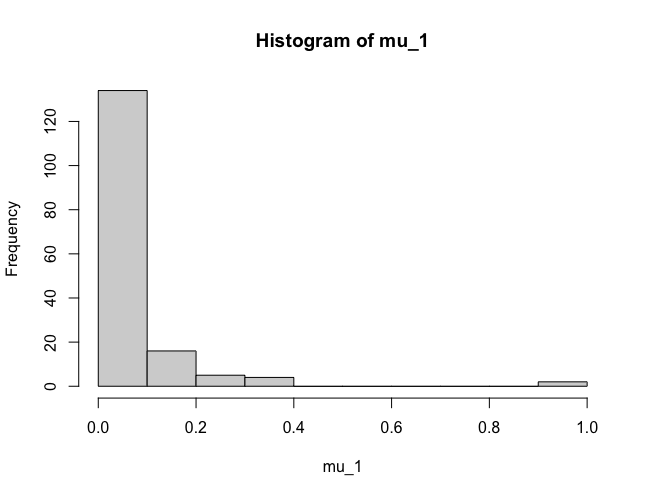
\includegraphics[width=\linewidth]{Histogram of mu_1 twitter15.png}
    \caption{Histogram of $\mu_1$ values for first time period for \textit{Twitter18}}
    \label{fig:Hist mu_1 Twitter18}
\endminipage\hfill
\minipage{0.32\textwidth}
  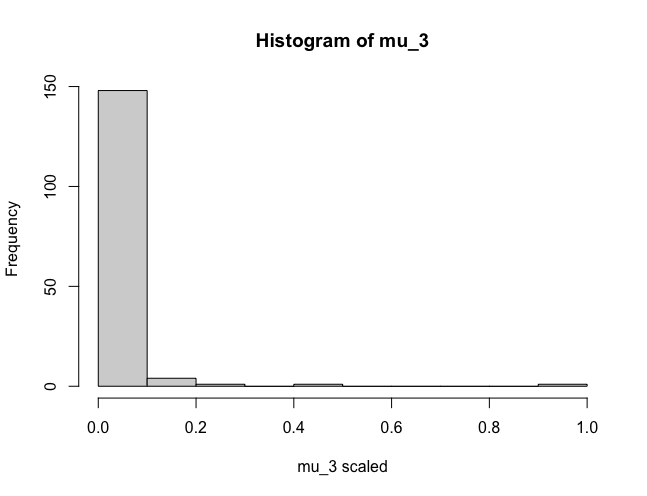
\includegraphics[width=\linewidth]{histogram_mu_3_scaled.png}
    \caption{Histogram of $\mu_3$ values for first time period for \textit{Twitter18}}
    \label{fig:Hist mu_3 Twitter18}
\endminipage\hfill
\minipage{0.32\textwidth}
  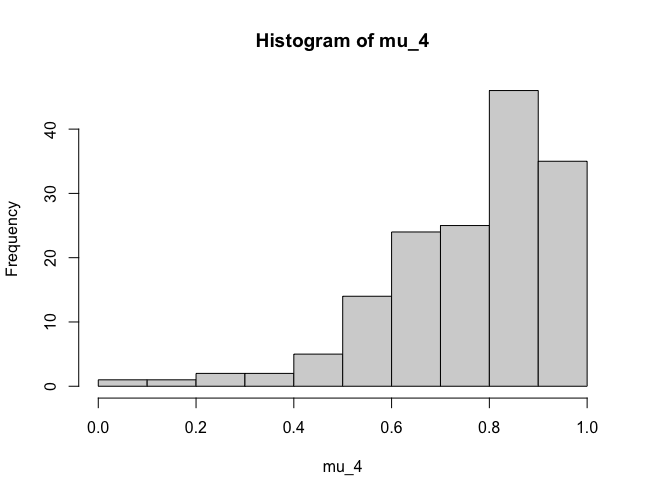
\includegraphics[width=\linewidth]{histogram of mu_4.png}
    \caption{Histogram of $\mu_4$ values for first time period for \textit{Twitter18}}
    \label{fig:Hist mu_4 Twitter18}
\endminipage
\end{figure}
Results for $\mu_6$:
Because these tweets all ``started" at the same time, $\mu_6$ was less informative than the other three. However, the $v_c$ value at $j=1$ was 0.89, which implies that around 89\% of all tweets need to be checked. 89\% is far too large of a number to consistently check as there are more than 500 million tweets per day \cite{raffi2013tweets}, which would require 445 million fact checks per day. That is unsustainable. However, it's important to recognize that 89\% is for \textbf{total} vaccination of the \textit{entire} network.

In this experiment, though, $\mu_6$ saw steady decrease in each time period (Fig. \ref{fig:mu6 Twitter18}), which implies that this algorithm did successfully remove the ``super spreaders" first. In fact, when $j=1$, $\langle v_c \rangle = 0.894$, but by $j=24$, $\langle v_c \rangle = 0.091$. That is a substantial decrease.
\begin{figure}[h!]
    \centering
    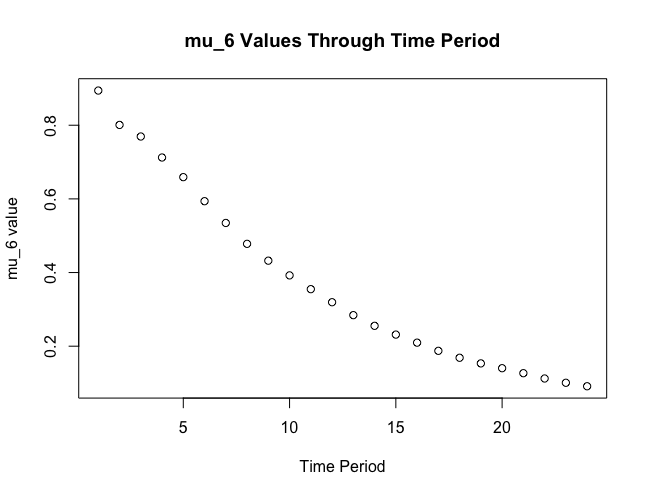
\includegraphics[width=8cm]{mu6 graph.png}
    \caption{Plot of $\mu_6$ values for each time period in \textit{Twitter18}}
    \label{fig:mu6 Twitter18}
\end{figure}

Even setting $\langle \rho_{\Delta} \rangle$ to 0.5, highly partisan content still rose to the top of this list. 10 out of the 24 tweets that the algorithm selected are partisan in nature(Tweets 1, 2, 3, 4, 6, 8, 9, 15, 17, 18), 1 is clearly spam (Tweet 22), and 2 are news that need to be fact-checked (Tweets 7 and 14). Arguably, it is worthwhile for tweets surrounding celebrity deaths (Tweets 11, 16, and 21) to be fact-checked even though they aren't partisan in nature, since death hoaxes are a common source of fake news \cite{moses2017celebrity}.

It correctly vaccinated Tweet 1 first (``and @abc, please tweet saying that you did not pay or compensate darren wilson for the interview in any way. we're waiting. \#ferguson"), as it had high values for $\mu_1$, $\mu_2$, $\mu_3$, and $\mu_4$: it came from a source with a high number of followers, focused on one of the top 10 bigrams (Darren Wilson was the officer who shot Michael Brown in Ferguson, MO \cite{halpern2015cop}), and was spreading quickly. The $v_c$ for this tweet at $j=1$ was 0.9959 -- almost every single node would have to be vaccinated or immunized in order to prevent this post from spreading. This charge by @deray is exactly the sort of tweet that should be checked first: it's on a controversial topic, it's \textit{sythetic a posteriori} knowledge, it's partisan, and could muddy the waters of discussion on the topic. 

\subsection{PHEME Data Set}
The PHEME data set \cite{kochkina2018pheme} is made up of 105,354 tweets and 7,442 source tweets. A source tweet is defined as a tweet where the ``in$\_$reply$\_$to$\_$status$\_$id" field in the twitter API JSON field is null. 

These tweets cover nine events - five actual and four rumors: the 2014 unrest in Ferguson after the shooting of Michael Brown, the 2014 shooting in Ottawa where a Canadian soldier died, the 2014 siege of the Lindt chocolate caf{\'e} in Sydney by a gunman, the 2015 shooting of journalists at the Charlie Hebdo newspaper, the 2015 crash of the Germanwings airplane between Barcelona and D\"{u}sseldorf, the 2014 rumor that Prince would play a concert in Toronto, the 2014 rumor that the Bern Museum of Fine Arts would accept art from the son of a Nazi art dealer, the 2015 rumor that something had happened to Vladimir Putin after he was ``missing" for 10 days, the 2014 rumor that AC Milan footballer Michael Essien had contracted Ebola.

\subsubsection{Data Analysis}
The \textit{PHEME} set also follows a somewhat normal distribution of the $\log_{10}|Y|$ and $\log_{10}|Z|$ with a $\gamma_{in} = 3.2$ and a $\gamma_{out} = 1.02$. The $\gamma_{in}$ is larger than in the Arapacio set (2.2) and the \textit{Twitter15} set (2.6), yet it still falls within the boundaries of a scale free network. If anything, this set more closely aligns with a typical scale-free network, as $\gamma = 3$ is the standard value for the Barab{\'a}si-Albert model \cite{barabasi1999emergence,barabasi2000scale,pastor2001epidemic}.

As expected, the $\mu_2$ values aligned closely to the topics; however, the distribution of bigrams is not proportional to the number of tweets: Charlie Hebdo tweets make up 29\% of the tweets, but are only 20\% of the top bigrams, while the Ottawa Shooting was 12\% of the tweets but 30\% of the bigrams.

At the same time, it is important to recognize how many tweets use only two Charlie Hebdo bigrams - those two appear 519 times, while the Ottawa Shooting bigrams appear 351 times and the Ferguson Shooting bigrams appear 416 times. A future course of study could be to analyze if there are underlying reasons why a particular topic might be more or less prone to having multiple smaller bigram variations vs. one large and consistent bigram.

Perhaps this can provide a non-malicious explanation to the charges of censorship provided by Tufecki and Lotan (Sec. \ref{sec: what is being shared}): individuals talking about the death of Freddie Gray will likely use a combination of phrases to describe this topic (freddie, gray; baltimore,grey; police, brutality; etc.) whereas all tweets on the ice bucket challenge will likely feature two bigrams (ice bucket, bucket challenge). A human could probably piece together all of the Freddie Gray bigrams as being related to a single topic, but a neural network could not.

\subsubsection{Results}
An examination of the $\mu_6$ metric over the time period (Fig. \ref{fig:mu6 PHEME}) shows that the algorithm was successful. While it did not catch every piece of misinformation (the false article by the Daily Mail in tweet Fig. \ref{fig:Daily Mail Tweet, Jan 7, 2015} was not fact-checked by this algorithm), those posts reached dead-ends so quickly that they did not need to be fact checked. This data set went from $v_c = 0.7$ when $j = 1$ to $v_c = 0$ when $j = 24$. Because the drop off was so steep, this experiment was re-run with $j$ being in 3 second increments for the first minute (20 total time steps):

\begin{figure}[h]
\centering
\minipage{0.32\textwidth}
  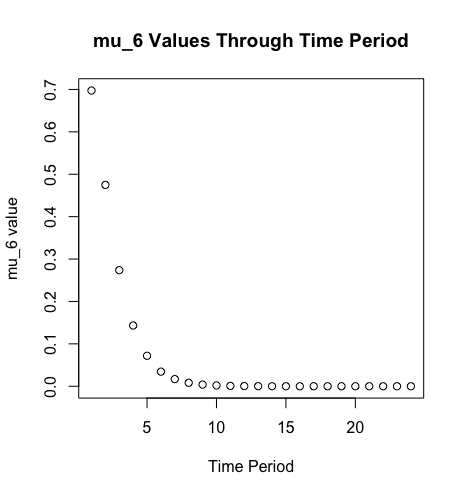
\includegraphics[width=\linewidth]{mu_6 pheme.png}
      \caption{Plot of $\mu_6$ values for each time period in \textit{PHEME} set}
    \label{fig:mu6 PHEME}
\endminipage\hfill
\minipage{0.32\textwidth}
  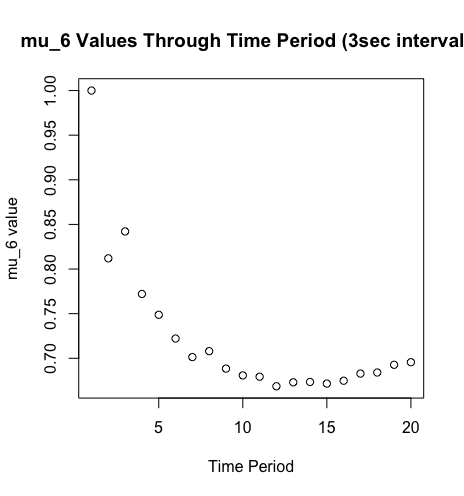
\includegraphics[width=\linewidth]{mu_6 3 second intervals through one minute.png}
    \caption{Plot of $\mu_6$ values for each time period in \textit{PHEME} set, 3 second intervals up to 1 minute}
    \label{fig:mu6 PHEME 3s}
\endminipage
\end{figure}

The algorithm continues to succeed in dropping the $v_c$ rate at a rapid pace from 1 to 0.67. The $v_c$ rate rebounds up to approximately 0.7 at 1 minute, but it is still lower then where it begins. Given the sporadic nature of tweets and the incomplete nature of this data set, it is not surprising that $v_c$ when $j=0.15$ is greater than when $j = 0.1$. 

\section{Conclusion}
The goal of this article was to provide a framework by which a fact checking team could maximize their resources and combat fake news in a scalable fashion. This solution has been provided. Unlike other fake news detection processes, it is adaptable to the user in question (Eq. \ref{mu_1 equation}), it factors in the importance of a topic on a given day (Eq. \ref{mu_2 equation}), it includes epidemic spreading rate of that particular tweet (Eq. \ref{mu_3 equation}), it de-prioritizes content at the end of its lifespan (Eq. \ref{mu_4 and mu_5}), and it provides a global KPI for the team to benchmark their successes (Eq. \ref{mu_4 and mu_5}).

From an epistemological standpoint, this article breaks down statements into various categories with assigned possible $\tau$ values, to separate content that machine learning is uniquely suited for and content that it is not. This is a stumbling block for global RNN solutions as they struggle with posts that are vague, hyperbolic, ironic, sarcastic, etc. This article makes no judgment about truth values, therefore there is no fear that an ironic statement will be deemed false. 

Visualizing this problem as an epidemic spread instead of a machine learning problem further allows for a recognition that not every node is susceptible to each particular strain of fake news (Eq. \ref{immunity equation}). It provides for the problem of echo-chambers (Sec. \ref{sec: echo-chambers}) by factoring in partisanship into the Barab{\'a}si-Albert preferential attachment equation (Eq. \ref{Pdotpartisan}) and recognizing that highly partisan environments are breeding grounds for malicious actors. These issues of partisanship are included in $\tilde{\psi}$ and in the calculation of $u^*$'s. This allows for posts to be ranked according to communal susceptibility, whereas other solutions offer only blanket solutions based on text patterns and user information patterns. 

This solution is easily repeatable on a daily basis. By using moving averages for content with a half-life, topics that were relevant last week but not this week fall off and are replaced by more significant topics. By including the moving variance as well, topics that have typically low volumes but then see large spikes, such as the preparation for the January 6th insurrection at the U.S. Capitol \cite{Levenson2021capitol}, would be caught by this metric. 

By not attempting to catch every error and fact-check every post, the resources here are maximized. Most tweets quickly reach a dead end and have no further spread; spending any time checking them is wasted effort. 

Finally, the resources required for this are far lower than those needed for an RNN that would attempt to check all of the 550 million tweets written per day. Many of these underlying numbers, such as $|\psi|$ values for each user, are relatively static and easily selected from the available data layers. The equations using those numbers are far less resource intensive than the perpetual training and implementation of a CNN or RNN. As mentioned in \ref{what is being shared summary}, yesterday's topics are not the same as today's topics; text/user patterns that the neural networks detected yesterday are easily changed today. That will require constant training, which will be heavily resource intensive. This article solves that.

The next steps for validating this algorithm would be to use a much larger data set on computers with more sophisticated resources. Every piece of coding for this article was performed on a 2020 MacBook Air with only 8GB of RAM. Server level machines would be able to run this exact same algorithm much faster, and would be able to process the $\approx 6,366$ tweets that are posted every second on average. 

After that, the next step would be to determine the $\beta$ weights for each $\mu$ value. For this article, every $\mu$ value was transformed using minmax, which made every $\mu$ value equally important. The inclusion of $\beta$ weights will allow for platforms to adjust the importance of metrics as needed and may be recalibrated on an iterative basis until the optimal values are discovered.



\newpage
\bibliographystyle{elsarticle-num-names} 
\bibliography{bibliography}


\end{document}

\endinput
